%%% Hlavní soubor. Zde se definují základní parametry a odkazuje se na ostatní části. %%%

%% Verze pro jednostranný tisk:
% Okraje: levý 40mm, pravý 25mm, horní a dolní 25mm
% (ale pozor, LaTeX si sám přidává 1in)
\documentclass[12pt,a4paper]{report}
\setlength\textwidth{145mm}
\setlength\textheight{247mm}
\setlength\oddsidemargin{15mm}
\setlength\evensidemargin{15mm}
\setlength\topmargin{0mm}
\setlength\headsep{0mm}
\setlength\headheight{0mm}
% \openright zařídí, aby následující text začínal na pravé straně knihy
\let\openright=\clearpage

%% Pokud tiskneme oboustranně:
% \documentclass[12pt,a4paper,twoside,openright]{report}
% \setlength\textwidth{145mm}
% \setlength\textheight{247mm}
% \setlength\oddsidemargin{14.2mm}
% \setlength\evensidemargin{0mm}
% \setlength\topmargin{0mm}
% \setlength\headsep{0mm}
% \setlength\headheight{0mm}
% \let\openright=\cleardoublepage

% Přepneme na českou sazbu
\usepackage[slovak]{babel}
\usepackage[IL2]{fontenc}

%% Použité kódování znaků: obvykle latin2, cp1250 nebo utf8:
\usepackage[utf8]{inputenc}

%%% Další užitečné balíčky (jsou součástí běžných distribucí LaTeXu)
\usepackage{amsmath}        % rozšíření pro sazbu matematiky
\usepackage{amsfonts}       % matematické fonty
\usepackage{amsthm}         % sazba vět, definic apod.
\usepackage{bbding}         % balíček s nejrůznějšími symboly
			    % (čtverečky, hvězdičky, tužtičky, nůžtičky, ...)
\usepackage{bm}             % tučné symboly (příkaz \bm)
\usepackage{graphicx}       % vkládání obrázků
\usepackage{fancyvrb}       % vylepšené prostředí pro strojové písmo
\usepackage{indentfirst}    % zavede odsazení 1. odstavce kapitoly
\usepackage{natbib}         % zajištuje možnost odkazovat na literaturu
			    % stylem AUTOR (ROK), resp. AUTOR [ČÍSLO]
\usepackage[nottoc]{tocbibind} % zajistí přidání seznamu literatury,
                            % obrázků a tabulek do obsahu
\usepackage{icomma}         % inteligetní čárka v matematickém módu
\usepackage{dcolumn}        % lepší zarovnání sloupců v tabulkách
\usepackage{booktabs}       % lepší vodorovné linky v tabulkách
\usepackage{paralist}       % lepší enumerate a itemize
\usepackage[usenames]{xcolor}  % barevná sazba
\usepackage{float}

\usepackage{subcaption}
\usepackage[noend]{algpseudocode}
\usepackage{algorithm}
\usepackage{cases}
\usepackage{tikz}
\usepackage{amssymb}
\usetikzlibrary{decorations.pathmorphing} % noisy shapes
\usetikzlibrary{fit}					% fitting shapes to coordinates
\usetikzlibrary{backgrounds}	% drawing the background after the foreground

%%% Údaje o práci

% Název práce v jazyce práce (přesně podle zadání)
\def\NazevPrace{Vizualizace sekundární struktury RNA s využitím existujících struktur}

% Název práce v angličtině
\def\NazevPraceEN{RNA secondary structure visualization using existing structures}

% Jméno autora
\def\AutorPrace{Richard Eliáš}

% Rok odevzdání
\def\RokOdevzdani{2016}

% Název katedry nebo ústavu, kde byla práce oficiálně zadána
% (dle Organizační struktury MFF UK, případně plný název pracoviště mimo MFF)
\def\Katedra{Katedra softwarového inženýrství}
\def\KatedraEN{Department of Software Engineering}

% Jedná se o katedru (department) nebo o ústav (institute)?
\def\TypPracoviste{Katedra}
\def\TypPracovisteEN{Department}

% Vedoucí práce: Jméno a příjmení s~tituly
\def\Vedouci{RNDr. David Hoksza, Ph.D.}

% Pracoviště vedoucího (opět dle Organizační struktury MFF)
\def\KatedraVedouciho{Katedra softwarového inženýrství}
\def\KatedraVedoucihoEN{Department of Software Engineering}

% Studijní program a obor
\def\StudijniProgram{Informatika}
\def\StudijniObor{Obecná informatika}

% Nepovinné poděkování (vedoucímu práce, konzultantovi, tomu, kdo
% zapůjčil software, literaturu apod.)
\def\Podekovani{%
Poděkování.
}

% Abstrakt (doporučený rozsah cca 80-200 slov; nejedná se o zadání práce)
\def\Abstrakt{%
Abstrakt .. TODO
}
\def\AbstraktEN{%
RNA secondary structure data, both experimental and predicted, are becoming increasingly
available which is reflected in the increased demand for tools enabling their analysis. The common first step
in the analysis of RNA molecules is visual inspection of their secondary structure. In order to correctly lay
out an RNA structure, the notion of optimal layout is required. However, optimal layout of RNA structure has
never been formalized and is largely habitual. To tackle this problem we propose an algorithm capable of
visualizing an RNA structure using a related structure with a well-defined layout. The algorithm first
converts both structures into a tree representation and then uses tree-edit distance algorithm to find out
the minimum number of tree edit operations to convert one structure into the other. We couple each tree
edit operation with a layout modification operation which is then used to gradually transform the known
layout into the target one. The optimality of tree edit distance algorithm causes that the common motives
are retained and the regions which differ in both the structures are taken care of. Visual inspection and
planarity evaluation reveals that the algorithm is able to give good layouts even for relatively distant
structures while keeping the layout planar. The new method is well suited for situations when one needs to
visualize a structure for with a homologous structure with a good visualization is already available.
}

% 3 až 5 klíčových slov (doporučeno), každé uzavřeno ve složených závorkách
\def\KlicovaSlova{%
{TODO}
{klíčová} {slova}
}
\def\KlicovaSlovaEN{%
RNA secondary structure, visualization, homology
}

%% Balíček hyperref, kterým jdou vyrábět klikací odkazy v PDF,
%% ale hlavně ho používáme k uložení metadat do PDF (včetně obsahu).
\usepackage[pdftex,unicode]{hyperref}   % Musí být za všemi ostatními balíčky
\hypersetup{breaklinks=true}
\hypersetup{pdftitle={\NazevPrace}}
\hypersetup{pdfauthor={\AutorPrace}}
\hypersetup{pdfkeywords=\KlicovaSlova}
\hypersetup{urlcolor=blue}

%% Definice různých užitečných maker (viz popis uvnitř souboru)
%%% Tento soubor obsahuje definice různých užitečných maker a prostředí %%%
%%% Další makra připisujte sem, ať nepřekáží v ostatních souborech.     %%%

%%% Drobné úpravy stylu

% Tato makra přesvědčují mírně ošklivým trikem LaTeX, aby hlavičky kapitol
% sázel příčetněji a nevynechával nad nimi spoustu místa. Směle ignorujte.
\makeatletter
\def\@makechapterhead#1{
  {\parindent \z@ \raggedright \normalfont
   \Huge\bfseries \thechapter. #1
   \par\nobreak
   \vskip 20\p@
}}
\def\@makeschapterhead#1{
  {\parindent \z@ \raggedright \normalfont
   \Huge\bfseries #1
   \par\nobreak
   \vskip 20\p@
}}
\makeatother

% Toto makro definuje kapitolu, která není očíslovaná, ale je uvedena v obsahu.
\def\chapwithtoc#1{
\chapter*{#1}
\addcontentsline{toc}{chapter}{#1}
}

% Trochu volnější nastavení dělení slov, než je default.
\lefthyphenmin=2
\righthyphenmin=2

% Zapne černé "slimáky" na koncích řádků, které přetekly, abychom si
% jich lépe všimli.
\overfullrule=1mm

%%% Makra pro definice, věty, tvrzení, příklady, ... (vyžaduje baliček amsthm)

\theoremstyle{plain}
\newtheorem{veta}{Veta}
\newtheorem{lemma}[veta]{Lemma}
\newtheorem{tvrz}[veta]{Tvdenie}

\theoremstyle{plain}
\newtheorem{definice}{Definícia}

\theoremstyle{remark}
\newtheorem*{dusl}{Dôsledok}
\newtheorem*{pozn}{Poznámka}
\newtheorem*{prikl}{Príklad}

%%% Prostředí pro důkazy

\newenvironment{dukaz}{
  \par\medskip\noindent
  \textit{Dôkaz}.
}{
\newline
\rightline{$\square$}  % nebo \SquareCastShadowBottomRight z balíčku bbding
}

%%% Prostředí pro sazbu kódu, případně vstupu/výstupu počítačových
%%% programů. (Vyžaduje balíček fancyvrb -- fancy verbatim.)

\DefineVerbatimEnvironment{code}{Verbatim}{fontsize=\small, frame=single}

%%% Prostor reálných, resp. přirozených čísel
\newcommand{\R}{\mathbb{R}}
\newcommand{\N}{\mathbb{N}}

%%% Užitečné operátory pro statistiku a pravděpodobnost
\DeclareMathOperator{\pr}{\textsf{P}}
\DeclareMathOperator{\E}{\textsf{E}\,}
\DeclareMathOperator{\var}{\textrm{var}}
\DeclareMathOperator{\sd}{\textrm{sd}}

%%% Příkaz pro transpozici vektoru/matice
\newcommand{\T}[1]{#1^\top}

%%% Vychytávky pro matematiku
\newcommand{\goto}{\rightarrow}
\newcommand{\gotop}{\stackrel{P}{\longrightarrow}}
\newcommand{\maon}[1]{o(n^{#1})}
\newcommand{\abs}[1]{\left|{#1}\right|}
\newcommand{\dint}{\int_0^\tau\!\!\int_0^\tau}
\newcommand{\isqr}[1]{\frac{1}{\sqrt{#1}}}

%%% Vychytávky pro tabulky
\newcommand{\pulrad}[1]{\raisebox{1.5ex}[0pt]{#1}}
\newcommand{\mc}[1]{\multicolumn{1}{c}{#1}}

\renewcommand{\O}[1]{\ensuremath{\mathcal{O}}(#1)}



%% Titulní strana a různé povinné informační strany
\begin{document}
%%% Titulní strana práce a další povinné informační strany

%%% Titulní strana práce

\pagestyle{empty}
\hypersetup{pageanchor=false}

\begin{center}

\centerline{\mbox{\includegraphics[width=166mm]{../img/logo-cs.pdf}}}

\vspace{-8mm}
\vfill

{\bf\Large BAKALÁŘSKÁ PRÁCE}

\vfill

{\LARGE\AutorPrace}

\vspace{15mm}

{\LARGE\bfseries\NazevPrace}

\vfill

\Katedra

\vfill

\begin{tabular}{rl}

Vedoucí bakalářské práce: & \Vedouci \\
\noalign{\vspace{2mm}}
Studijní program: & \StudijniProgram \\
\noalign{\vspace{2mm}}
Studijní obor: & \StudijniObor \\
\end{tabular}

\vfill

% Zde doplňte rok
Praha \RokOdevzdani

\end{center}

\newpage

%%% Následuje vevázaný list -- kopie podepsaného "Zadání bakalářské práce".
%%% Toto zadání NENÍ součástí elektronické verze práce, nescanovat.

%%% Strana s čestným prohlášením k bakalářské práci

\openright
\hypersetup{pageanchor=true}
\pagestyle{plain}
\pagenumbering{roman}
\vglue 0pt plus 1fill

\noindent
Prohlašuji, že jsem tuto bakalářskou práci vypracoval(a) samostatně a výhradně
s~použitím citovaných pramenů, literatury a dalších odborných zdrojů.

\medskip\noindent
Beru na~vědomí, že se na moji práci vztahují práva a povinnosti vyplývající
ze zákona č. 121/2000 Sb., autorského zákona v~platném znění, zejména skutečnost,
že Univerzita Karlova má právo na~uzavření licenční smlouvy o~užití této
práce jako školního díla podle §60 odst. 1 autorského zákona.

\vspace{10mm}

\hbox{\hbox to 0.5\hsize{%
V ........ dne ............
\hss}\hbox to 0.5\hsize{%
Podpis autora
\hss}}

\vspace{20mm}
\newpage

%%% Povinná informační strana bakalářské práce

\openright

\vbox to 0.5\vsize{
\setlength\parindent{0mm}
\setlength\parskip{5mm}

Název práce:
\NazevPrace

Autor:
\AutorPrace

\TypPracoviste:
\Katedra

Vedoucí bakalářské práce:
\Vedouci, \KatedraVedouciho

Abstrakt:
\Abstrakt

Klíčová slova:
\KlicovaSlova

\vss}\nobreak\vbox to 0.49\vsize{
\setlength\parindent{0mm}
\setlength\parskip{5mm}

Title:
\NazevPraceEN

Author:
\AutorPrace

\TypPracovisteEN:
\KatedraEN

Supervisor:
\Vedouci, \KatedraVedoucihoEN

Abstract:
\AbstraktEN

Keywords:
\KlicovaSlovaEN

\vss}

\newpage

%%% Poděkování

\openright

\noindent
\Podekovani

\newpage

\openright
\pagestyle{plain}
\pagenumbering{arabic}
\setcounter{page}{1}


%%% Strana s automaticky generovaným obsahem bakalářské práce

\tableofcontents

%%% Jednotlivé kapitoly práce jsou pro přehlednost uloženy v samostatných souborech
%
\chapter*{Úvod}
\addcontentsline{toc}{chapter}{Úvod}

Donedávna sa myslelo, že úloha ribonukleovej kyseliny, RNA, je obmedzená
iba na syntézu bielkovín, buď ako nositeľka genetickej informácie (mRNA),
alebo ako prenášač aminokyselín pri ich tvorbe (tRNA).
Avšak existuje mnoho ďalších druhov, od relatívne malých molekúl majúcich
iba desiatky nukleotidov, ktoré ovplyvňujú expresiu génov
(miRNA, siRNA, snRNA, snoRNA a~ďalšie) (\citet{RNA_MI_SI}, \citet{RNA_SN_SNO}),
až po veľké molekuly s~tisíckami nukleotidov, ktoré sa podieľajú na tvorbe ribozómu (rRNA).

Spolu s~objavmi ďalších funkcií RNA molekúl rastie záujem o~nástroje dovoľujúce
študovať ich štruktúru.
Primárna štruktúra je určená poradím nukleotidov v~reťazci RNA.
Terciárnu štruktúru získame ich priestorovým usporiadaním.
Poslednou a~v~tejto práci pre nás najdôležitejšou
bude sekundárna štruktúra. Tú reprezentuje zoznam nukleotidov ktoré sú spojené väzbou.
Spárované nukleotidy sú blízko seba v~priestore a~tak nám sekundárna relatívne
dobre aproximuje terciárnu štruktúru. Predpovedanie terciárnej štruktúry nieje veľmi
spoľahlivé ani pre kratšie molekuly. Naopak, pre menšie molekuly a~ich  sekundárnu
štruktúru existujú spoľahlivejšie metódy. Ich prehľad a~porovnanie nájdeme v~článku
od autorov \citet{SEC_STR_PREDICT_TOOLS}.
Príbuzné štruktúry nám vedia poslúžiť k predpovedaniu konzervovaných častí, dokonca
aj veľkých rRNA molekúl (\citet{SEC_STR_PREDICTION}).

Vizualizácia sekundárnej štruktúry RNA sa dá previesť na kreslenie grafu,
ktorého vrcholy tvoria nukleotidy a~hrany reprezentujú páry medzi nimi.
Kreslenie grafov je značne preskúmanou témou, keďže nachádza uplatnenie vo veľa
doménach, ako napríklad analýza sociálnych sietí (\citet{SOCIAL_NETWORK_ANALYSIS})
alebo vo všeobecnej analýze dát (\citet{GRAPH_DRAWING}).

Cieľom vizualizácie sekundárnej štruktúry RNA je zachytit párovanie nukleotidov
v~molekule a~ideálne všetky ďalšie motívy, ktoré sa v~štruktúre vyskytujú,
ako napríklad hairpin, bulge, interior a~multi-branch loop.
Existujúce nástroje na vizualizáciu zväčša volia medzi tromi tipmi reprezentácie
štruktúry (\citet{JVIZ}): spojnicový graf (linked graph), kruhový graf (circular graph)
alebo štandardná štruktúra (classical structure).
Aj keď spojnicový a~kruhový graf podporujú vizualizáciu párovania báz, motívy
sa v~nej dajú nájsť len veľmi ťažko, ak vôbec.
Preto nám na hľadanie motívov v~RNA ostala štandardná reprezentácia štruktúry RNA.
Bolo vymyslených množstvo riešení -
RNAfold z~balíka ViennaRNA (\citet{VIENNA_RNA}), VARNA (\citet{VARNA}),
RnaViz (\citet{RNA_VIZ}), jViz.RNA (\citet{JVIZ}), mfold (\citet{MFOLD}),
PseudoViewer (\citet{PSEUDOVIEWER}) alebo RNAView (\citet{RNAVIEW}).
Avšak iba niektoré z týchto nástrojov a algoritmov sú použiteľné pre vizualizáciu
veľkých štruktúr, akou sú napríklad podjednotky rRNA (RNAfold, RnaViz a RNAView).
Porovnanie väčšiny z nich nájdeme v článku autorov \citet{DRAWING_COMPARISION}.

Vzhľadom k~tomu, že je nekonečne mnoho možností ako rozložiť sekundárnu štruktúru,
potrebujeme zistiť aké kritéria by malo nakreslenie RNA spĺňať. Nanešťastie
tieto kritéria niesú formalizované, avšak niektoré vlastnosti ako napríklad
rovinnosť nakreslenia, kreslenie loopov (hairpin, bulge, interior a multi-branch)
na kružnice a~vrcholy stemu ležiace na jednej priamke sú spoločné pre väčšinu
vizualizácii používaných vo vedeckej komunite, ako popisujú \citet{RNA_DRAW}.
Ostatné sa prispôsobujú oblasti štúdia, kvôli čomu každý algoritmus nebude
vyhovovať veľkej časti používateľov.
Dôvod môžeme ilustrovať na ribozomálnej RNA. Štruktúry týchto molekúl
majú veľké konzervované časti, ktoré biológovia očakávajú na rovnakom mieste
na obrázku, vďaka čomu sa vedia orientovať aj v~relatívne veľkej molekule
a~môžu skúmať a~nachádzať tie menej konzervované časti, ktoré sa líšia medzi organizmami.
To znamená, že ak chceme štruktúru vizualizovať, potrebujeme ukladať
konzervované časti vždy na rovnaké miesto v~obrázku.

Potreba vizualizácie, ktorá by zachovávala čo najviac spomínaných vlastností
nás viedla k~vytvoreniu nového vizualizačného algoritmu založeného
na použití šablónovej (vzorovej) molekuly (\citet{ELIAS_HOKSZA}).
Algoritmus na vstupe vezme cieľovú
štruktúru, ktorú chceme vizualizovať a~inú, podobnú štruktúru u~ktorej poznáme jej
nakreslenie. Túto podobnú molekulu nazývame šablónou. Obe štruktúry sú
prevedené do ich stromovej reprezentácie. Následne nájdeme najkratšiu postupnosť
editačných operácií, ktoré prevedú strom molekuly šablónovej na vizualizovanú
molekulu a~rovnako menia aj nakreslenie šablóny na nakreslenie cieľovej molekuly.
Vzhľadom k~tomu, že editačné operácie ktoré menia nakreslenie odpovedajú
minimálnej editačnej vzdialeností medzi stromami, nakreslenie spoločných častí sa nemení.
Táto metóda je teda schopná vizualizovať sekundárnu štruktúru RNA
molekuly presne podľa zvyku biológov - podľa poskytnutého vzorového nakreslenia.



%\include{ted_priklad}
%\renewcommand{\SS}{\mathbb{S}}
\newcommand{\Par}[2]{\mbox{$( #1, #2 )$}}

\chapter{Uvod do studia struktury RNA}

Na zaciatku prace strucne zoznamime citatela s pojmamy, ktore s RNA a jej strukturou suvisia.

\section{Co je RNA}

Nositelkami genetickej informacie bunky su molekuly nukleovych kyselin
tvorene retazcami nukleotidov, ktore su zakladnymi stavebnymi jednotkami
nukleovych kyselin. Vyskytuje sa niekolko variant nukleotidov (baz). U RNA su to
adein (A), guanin (G), cytozin (C), uracyl (U),
pri DNA sa namiesto uracylu vyskytuje tymin (T).
Medzi jednotlivymi bazami sa mozu vyskytovat vodikove vazby. Nukleotidy maju
vzajomnu preferenciu, co znamena, ze bazy vznikaju najcastejsie medzi A-U a C-G
u RNA a podobne A-T a C-G u DNA.
Medzi jednotlivymi bazami existuju vazby na principe komplementarity.
Vodikove vazby existuju medzi bazami A-U a C-G u RNA a podobne A-T a C-G u DNA.
Strukturu nukleovych kyselin mozeme chapat podla stupna zjednodusenia
\begin{itemize}
	\item Primarna struktura - je urcena poradim jednotlivych nukleotidov
		do polynukleotidoveho retazca
	\item Sekundarna struktura - je dana parovanim medzi bazami molekuly
	\item Terciarna struktura - 3D priestorove usporiadanie molekuly
\end{itemize}
DNA je dvojvlaknova molekula u ktorej spojenie medzi vlaknami sa realizuje na principe
komplementarity.
Naopak, RNA je iba jednovlaknova molekula a v snahe minimalizovat volnu energiu molekuly
sa paruje sama na seba. V tomto hraju rolu pritazlive sily medzi bazami.

V praci budeme strukturou mysliet prave sekundarnu strukturu RNA, ak nebude povedane inak.

Az donedavna sa myslelo, ze funkcia RNA je obmedzena na prenos genetickej informacie z DNA
v jadre bunky do ribozomu. Napriklad pri tvorbe bielkovin (mRNA), alebo transporter aminokyselin
v ribozome bunky (tRNA).
% TODO: citacie k druhom RNA
Avsak existuje mnoho dalsich, od relativne
malych molekul tvorenych desiatkami baz, ktore pomahaju pri expresii genov
(miRNA, siRNA, tmRNA a dalsie), az po velke, tvorene tisickami nukleotidov (rRNA).

\section{Sekundarna struktura rRNA + konzervovanost}

Ako hlavny objekt zaujmu sme si spomedzi vsetkych druhov RNA vybrali prave ribozomalnu,
najma kvoli jej velkosti a tomu, ze existujucim nastrojom prave velkost robi najvacsie problemy
pri vizualizacii.

\begin{definice}[Primarna struktura RNA]
  \label{def:RNA_primarna_struktura}
	Nech $\Sigma$ je abeceda $\{A, C, G, U\}$. Potom slovo $W \in \Sigma^n$ nad touto abecedou
	je sekvencia nukleotidov (baz) RNA.
\end{definice}

Jednotlive nukleotidy sekvencie RNA budeme, ak bude jasne o co ide, oznacovat priamo poradovym
cislom, teda $i$ bude oznacovat nukleotid $W_{i}$, resp. $W[i]$.

\begin{definice}[Sekundarna struktura RNA]
  \label{def:RNA_sekundarna_struktura}
	Nech $W$ je sekvencia podla definicie \ref{def:RNA_primarna_struktura} dlzky n.
	Sekundarnou strukturou oznacime mnozinu $\SS$ parov nukleotidov \Par{i}{j} takych, ze
	pre dva pary \Par{i}{j} a \Par{k}{l} $\in \SS$ (bez ujmy na obecnosti $i \leq k$)
  plati jedno z nasledujucich:
	\begin{itemize}
		\item $i = k \iff j = l$
		\item $i < j < k < l$, cize par \Par{i}{j} predchadza par \Par{k}{l}
		\item $i < k < l < j$, cize par \Par{i}{j} obsahuje par \Par{k}{l}
	\end{itemize}
\end{definice}

%TODO: obrazok prim/sek/terc struktury RNA

Prva podmienka zabezpecuje, ze nukleotid je najviac v jednom bazickom pare, druha a tretia
hovoria o usporiadani parov, bud su na sebe nezavisle alebo na seba nadvazuju.
Posledna podmienka zakazuje existenciu pseudouzlov (pseudoknots).

%TODO: pseudoknot obrazok
%TODO: 2 obrazky RNA napriec fylogenetickym stromom

\begin{figure}[H]
\centering
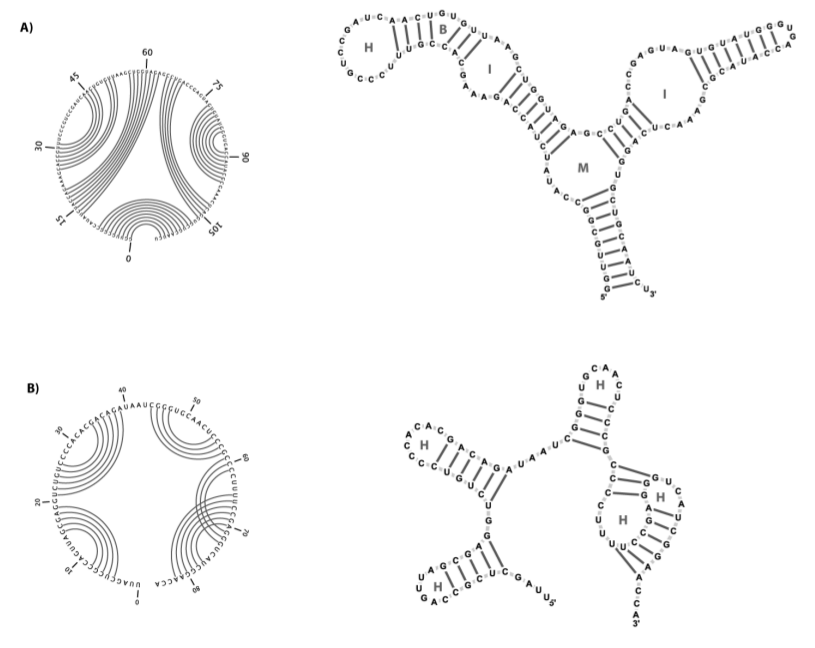
\includegraphics[width=140mm, height=120mm]{../img/RNA_circular_reprezentation.png}
\caption{Circular Feynman - kruhova reprezentacia sekundarnej struktury}
\label{obr:RNA_circular_representation}
\end{figure}


\subsection{Motivy}

Motivom v RNA mame na mysli casti molekuly, ktore vytvaraju urcite struktury.
Na obrazku \ref{obr:RNA_motifs} vidime motivy, ktore sa mozu v RNA vyskytovat.

Stem (stonka) je cast molekuly kde sa na seba paruju dva suvisle casti RNA vlakna.
Interior loop spaja dva stemy a medzi nimi na oboch stranach obsahuje nesparovane
bazy. Podobna je bulge (vypuklina), ale nesparovane nukleotidy ma iba z jednej strany.
Hairpin je medzi castami vlakna ktore sa paruju sami na seba.
Multibranch loop je podobna ako interior loop, ale spaja dokopy viac stemov.
V dalsom rozpravani nam bude stacit rozdelenie na stem a loop.

%TODO: ako nazyvat strukturne motivy v RNA: anglicky, alebo hladat vhodny preklad

\begin{figure}[H]
\centering
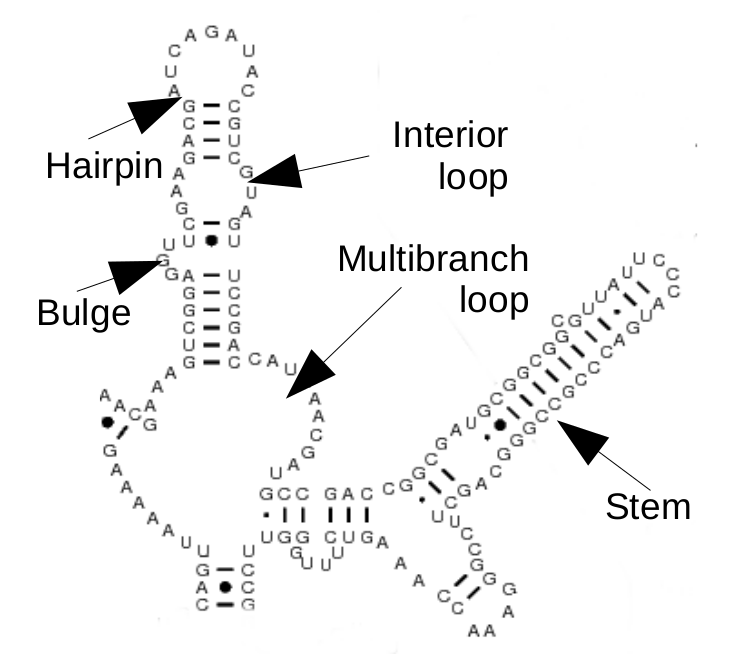
\includegraphics[width=70mm, height=70mm]{../img/struktury_v_rna.png}
\caption{Strukturalne motivy v RNA}
\label{obr:RNA_motifs}
\end{figure}


%
\chapter{Uvod a motivace}

Cielom prace je vytvorit program na vizualizaciu sekundarnej struktury RNA
pomocou uz existujucej vizualizacie inej molekuly.





%\usetikzlibrary{positioning, shapes, trees, graphs}

%rna, from 5' to 3':
% AUGCAAACUGGCACCCUCAU
% (((((...))(...))..))

\begin{center}
	\begin{tikzpicture}[
			baseline,
			level distance = 1.5 cm,
			basepair/.style = {ellipse, draw, minimum height = 0.3 cm, minimum width = 0.7 cm},
			unpaired/.style = {circle, draw, minimum width = 0.3 cm},
			level 2/.style={sibling distance = 3 cm},
			level 3/.style={sibling distance = 4 cm},
			level 4/.style={sibling distance = 1.5 cm}
		]
		\node[basepair] {AU}
		child {
			node[basepair] {UA}
			child {
				node[basepair] {GC}
				child {
					node[basepair] {CG}
					child {
						node[basepair] {AU}
						child {
							node[unpaired] {A}
						}
						child {
							node[unpaired] {A}
						}
						child {
							node[unpaired] {C}
						}
					}
				}
				child {
					node[basepair] {GC}
					child {
						node[unpaired] {C}
					}
					child {
						node[unpaired] {A}
					}
					child {
						node[unpaired] {C}
					}
				}
			}
			child {
				node[unpaired] {U}
			}
			child {
				node[unpaired] {C}
			}
		}
		;
	\end{tikzpicture}
\end{center}

\begin{center}
	\begin{tikzpicture}[on grid, -latex,
			base/.style = {circle, draw, minimum width = 0.5 cm},
			ends/.style = {draw = none, fill = none}]

		%ends, 5' a 3'
		\node[ends] (5end) {5'};
		\node[ends] (3end) [right = of 5end] {3'};

		%stem
		\node[base] (StemLeft1) [below = of 5end] {A};
		\node[base] (StemRight1) [right = of StemLeft1] {U};
		\node[base] (StemLeft2) [below = of StemLeft1] {U};
		\node[base] (StemRight2) [right = of StemLeft2] {A};

		%bulge
		\node[base] (Bulge1) [below right = of StemRight2] {C};
		\node[base] (Bulge2) [below = of Bulge1] {U};

		%stem
		\node[base] (StemRight3) [below left = of Bulge2] {C};
		\node[base] (StemLeft3) [left = of StemRight3] {G};

		%left-branch
		\node[base] (LBranchLStem1) [below left = of StemLeft3] {C};
		\node[base] (LBranchRStem1) [below right = of LBranchLStem1] {G};
		\node[base] (LBranchLStem2) [below left = of LBranchLStem1] {A};
		\node[base] (LBranchRStem2) [below left = of LBranchRStem1] {U};

		%left-branch-hairpin
		\node[base] (LBranchHairpin1) [below left = of LBranchLStem2] {A};
		\node[base] (LBranchHairpin2) [below = of LBranchHairpin1] {A};
		\node[base] (LBranchHairpin3) [right = of LBranchHairpin2] {C};

		%right-branch
		\node[base] (RBranchRStem1) [below right = of StemRight3] {C};
		\node[base] (RBranchLStem1) [below left = of RBranchRStem1] {G};

		%right-branch-hairpin
		\node[base] (RBranchHairpin1) [below right = of RBranchLStem1] {C};
		\node[base] (RBranchHairpin2) [right = of RBranchHairpin1] {A};
		\node[base] (RBranchHairpin3) [below right = of RBranchRStem1] {C};

		\begin{scope}[-]
		%pair edges
			\path[very thick]
			(StemLeft1) edge (StemRight1)
			(StemLeft2) edge (StemRight2)
			(StemLeft3) edge (StemRight3)
			(LBranchLStem1) edge (LBranchRStem1)
			(LBranchLStem2) edge (LBranchRStem2)
			(RBranchLStem1) edge (RBranchRStem1)
			;
		%lines around molecule
			\path[color = gray]
			(StemLeft1) edge (StemLeft2)
			(StemLeft2) edge (StemLeft3)
			(StemLeft3) edge (LBranchLStem1)
			(LBranchLStem1) edge (LBranchLStem2)
			(LBranchLStem2) edge (LBranchHairpin1)
			(LBranchHairpin1) edge (LBranchHairpin2)
			(LBranchHairpin2) edge (LBranchHairpin3)
			(LBranchHairpin3) edge (LBranchRStem2)
			(LBranchRStem2) edge (LBranchRStem1)
			(LBranchRStem1) edge (RBranchLStem1)
			(RBranchLStem1) edge (RBranchHairpin1)
			(RBranchHairpin1) edge (RBranchHairpin2)
			(RBranchHairpin2) edge (RBranchHairpin3)
			(RBranchHairpin3) edge (RBranchRStem1)
			(RBranchRStem1) edge (StemRight3)
			(StemRight3) edge (Bulge2)
			(Bulge2) edge (Bulge1)
			(Bulge1) edge (StemRight2)
			(StemRight2) edge (StemRight1)
			;
		\end{scope}

		\begin{scope}
			% edges to ends
			\path[thick]
			(5end) edge (StemLeft1)
			(StemRight1) edge (3end)
			;
		\end{scope}
	\end{tikzpicture}
\end{center}


\newcommand{\Cdel}{\ensuremath{c_{del}}}
\newcommand{\Cins}{\ensuremath{c_{ins}}}
\newcommand{\Cupd}{\ensuremath{c_{upd}}}

\newcommand{\AfullDecomposition}{\ensuremath{\mathcal{A}}}
\newcommand{\FrelevantSubforests}{\ensuremath{\mathcal{F}}}
\newcommand{\pluseq}{\stackrel{+}{=}}
\newcommand{\AlgCase}{$\left\{\rule{0pt}{\baselineskip}\right.$\parbox{\textwidth}}

\newcommand{\rtedCostSum}[3]{\sum_{{#1}' \in #1 - \gamma^{#2}(#1)}cena({#1}', #3)}
\newcommand{\set}[1]{\ensuremath{\{#1\}}}


%indentation in code:
\algdef{SE}[SUBALG]{Indent}{EndIndent}{}{\algorithmicend\ }
\algtext*{Indent}
\algtext*{EndIndent}


\chapter{Mapovanie medzi RNA stromami}

Ako sme spomínali v predchádzajúcich častiach, biológovia očakávajú, že
podobné RNA molekuly (pozeráme na sekundárnu štruktúru) budú mať aj podobnú vizualizáciu.
To znamená, že nakreslenia sa majú líšiť iba v rozdielnych častiach.

Vieme už, že RNA a jej sekundárnu štruktúru vieme reprezentovať ako usporiadaný strom.
Táto kapitola nám dá návod, ako nájsť najmenší počet úprav, ktorý prevedie jeden strom
na iný. Vďaka tomu, že poznáme vizualizáciu jednej molekuly - vieme rozvrhnutie jej báz na
obrázku a dokážeme ju previesť na cieľovú molekulu, rovnaké štruktúry budú rovnako vizualizované.

To nás privádza k algoritmu tree-edit-distance, TED. Je obdobou Levenshteinového
string-edit-distance algoritmu \citenum{LEVENSHTEIN}.
Ten počíta editačnú vzdialenosť medzi dvomi reťazcami a transformuje
jeden reťazec na druhý.

Problém u reťazcov je špeciálnym prípadom TEDu, kedy nám stromy zdegenerovali
na cesty (spojový zoznam).

\section{Tree-edit-distance algoritmus}

Základ TED algoritmu je v rekurzivnom vzorci \ref{eq:ted}. Vzdialenosť medzi
stromami F a G, $\delta(F, G)$ je definovana ako minimálny počet editačných operácií,
ktoré z F urobia G. Používame štandardne editačné operácie - delete, insert, update.

\begin{figure}[H]
\centering
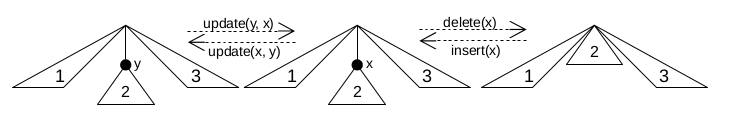
\includegraphics[width=140mm, height=30mm]{../img/TED_operations.png}
\caption{Ukážky TED operácií}
\label{obr:TED_operations}
\end{figure}

Delete, operácia zmazania vrcholu, znamená pripojiť k jeho predkovi všetkých jeho
potomkov so zachovaním poradia medzi nimi. Insert, vkladanie vrcholu, je opačná
operácia. Vkladáme vrchol medzi predka a nejakých jeho, po sebe nasledujúcich
potomkov. Update iba zmení hodnotu vo vrchole stromu.
Tieto operácie máme ukázané na obrázku \ref{obr:TED_operations}.

\begin{definice}[Editačná vzdialenosť]
  Nech F a G sú dva stromy. Editačna vzdialenosť (tree-edit-distance, $\delta(F, G)$),
	medzi F a G je rovná minimálnej cene, za ktorú strom F transformujeme na G.
\end{definice}

Rekurzia \ref{eq:ted} počíta vzdialenosť medzi dvoma lesmi $F$ a $G$.
\Cdel, \Cins a \Cupd sú ceny zmazania, vloženia a updatu vrcholu v strome
a $r_{F}$ a $r_{G}$ sú korene $F$, respektíve $G$ a to buď obidva najpravejšie
alebo najľavejšie (tzn. vyberieme najpravejší/najľavejší strom lesa a jeho koreň).


\begin{figure}
  \begin{subequations}
  \begin{align*}
    \begin{split}
    \delta(\emptyset, \emptyset) &=
      0
      \\
    \delta(F, \emptyset) &=
      \delta(F - r_{F}, \emptyset) + \Cdel(r_{F})
      \\
    \delta(\emptyset, G) &=
      \delta(\emptyset, G - r_{G}) + \Cins(r_{G})
    \end{split}
    \\[1ex]
    \delta(F, G) &=
      \begin{cases}
        \delta(F - r_{F}, G) + \Cdel(r_{F}) \\
        \delta(F, G - r_{G}) + \Cins(r_{G}) \\
        \delta(F - F_{r_{F}}, G - G_{r_{G}}) \\
          \quad \quad + \delta(F_{r_{F}} - r_{F}, G_{r_{G}} - r_{G}) \\
          \quad \quad + \Cupd(r_{F}, r_{G})
      \end{cases}
  \end{align*}
  \end{subequations}
  \caption{Rekurzívny vzorec pre výpočet tree-edit-distance od \citet{DMRW} a \citet{RTED}}
  \label{eq:ted}
\end{figure}


\section{\sloppy Vývoj algoritmu - rekurzia a dynamické programovanie}

Algoritmus TED prešiel vývojom postupne od \citet{TAI}, ktorý predstavil algoritmus
na výpočet editačnej vzdialenosti s priestorovou a časovou zložitosťou
\O{$m^3 \cdot n^3$}. Algoritmus vylepšili \citet{ZHANGSHASHA} vypozorovaním toho,
že nepotrebujeme počítať celú rekurziu. Ich algoritmus ma časovú zložitosť \O{$m^2 \cdot n^2$}
a priestorovú \O{$m \cdot n$}. \citet{KLEIN} dosiahol časovú zložitosť \O{$m^2 \cdot n \cdot \log{n}$},
avšak jeho riešenie potrebuje rovnako veľa pamäte.
\citet{DALUCQ} ukázali, že minimálny čas na beh algoritmu je \O{$m \cdot n \cdot \log{m} \cdot \log{n}$}.
\citet{DMRW} predstavili worst-case optimálny algoritmus pre tree-edit-distance.
Jeho časová a priestorová zložitosť je \O{$m^2 \cdot n \cdot (1 + \log{\frac{n}{m}})$} a
\O{$m \cdot n$}. \citet{RTED} ukázali spojitosť medzi efektivnosťou predchádzajúcich algoritmov
a tvarom stromov. Zovšeobecnili predchádzajúce prístupy a vytvorili algoritmus
s worst-case časom \O{$m^3$} a priestorom \O{$m \cdot n$}.
Ako dokázali, ich algoritmus je efektívny pre všetky tvary stromov a worst-case
prípad u neho nastane iba vtedy, ak lepší smer výpočtu neexistuje.

\subsection{RTED}

V nasledujúcich častiach sa budeme venovať výhradne algoritmu RTED od tvorcov \citet{RTED}.
Ich algoritmus rozdelíme na 2 časti, rovnako pomenovaný RTED a GTED.

RTED (Robust Tree Edit Distance) algoritmus bude pre nás algoritmus na výpočet
optimálnej dekompozičnej stratégie (viz definicia \ref{def:strategy})
a GTED (General Tree Edit Distance), algoritmus pre samotný výpočet editačnej
vzdialenosti z rekurzie \ref{eq:ted} s aplikovaním danej stratégie.

\begin{definice}[Dekompozičná stratégia]
  \label{def:strategy}
	Nech $F$ a $G$ sú lesy. Dekompozičná stratégia pre rekurziu \ref{eq:ted} priradí
  každej dvojici stromov $F_{v}$ a $G_{w}$ jednu cestu $\gamma_{T}$
  z koreňa do listu, kde $T \in \{F, G\}$.

	LRH dekompozičná stratégia vyberá vždy najľavejší/najpravejší/najťažší
	(left/right/heavy) vrchol až kým nepríde do listu. Najťažší vrchol je taký,
	v ktorého podstrome je najviac vrcholov. 
\end{definice}

To znamená, že dekompozičná stratégia nám pre dvojicu lesov povie,
ktorý z nich a akou cestou chceme rozložiť (dekomponovať).
V rekurzii to hovorí, či odoberám $r_{F}$, alebo $r_{G}$ vrchol.




\subsubsection{GTED: General Tree Edit Distance algoritmus}

Začneme princípom fungovania GTED algoritmu. Detaily pre LRH stratégie sú
v \citet{ZHANGSHASHA} pre left/right a v \citet{DMRW} pre heavy stratégiu.

\begin{definice}
  \label{def:relevant_subforests}
	Relevant subtrees stromu $F$ pre root-leaf cestu $\gamma$ sú stromy $F - \gamma$.

	Relevant subforests lesa $F$ pre nejakú root-leaf cestu $\gamma$ sú definované rekurzívne
  ($r_{R}$ a $r_{L}$ označujú najpravejší, respektíve najľavejší koreň $F$)
	\begin{align*}
    \mathcal{F}(\emptyset, \gamma) &= \emptyset
		\\
		\mathcal{F}(F, \gamma) &= \{F\} \cup
		\begin{cases}
      \mathcal{F}(F - r_{R}(F), \gamma), \quad{} &\text{ak $r_{L}(F) \in \gamma$}
			\\
      \mathcal{F}(F - r_{L}(F), \gamma), &\text{v ostatných pripadoch}
		\end{cases}
	\end{align*}
\end{definice}


\newcommand{\wi}{0.2\hsize}
\newcommand{\wit}{0.5\hsize}


\begin{figure}
    \begin{minipage}{\wi}
      \begin{tikzpicture}[
          on grid,
          font=\large,
          scale = \scale,
          level distance = 1.5 cm,
          every node/.style = {scale = \scale, circle, draw},
          tree/.style = {draw = none, fill = none}]

          \node[tree] (F) {F:};
          \node[right = of F] {4}
          child {
            node {2}
            child {
              node {1}
            }
          }
          child {
            node {3}
          }
          ;
      \end{tikzpicture}
    \end{minipage}
    \begin{minipage}{\wi}
      \begin{tikzpicture}[
          on grid,
          font=\large,
          scale = \scale,
          level distance = 1.5 cm,
          invisible/.style={opacity=0},
          every node/.style = {scale = \scale, circle, draw},
          tree/.style = {draw = none, fill = none}]

          \node[tree] (G) {G:};
          \node (3) [right = of G] {C}
          child {
            node {A}
            % nieje viditelny; je pridavany iba kvoli tomu, aby obidva stromy boli rovnako vysoke
            child[invisible] {
              node {I}
            }
          }
          child {
            node {B}
          }
          ;
      \end{tikzpicture}
    \end{minipage}
    \begin{minipage}{\wit}
      \begin{tabular}{c|c|c|c}
        \mc{$ForestDistance:$} & \mc{\subtree{\node{A};}} & \mc{\subtree{\node (A) {A}; \node[right = of A] {B};}} & \mc{\subtree{\node {C} child {node{A}} child {node{B}};}} \\
        \toprule
        \subtree{\node{1};}                                                 & 0 & 1 & 2 \\
        \midrule
        \subtree{\node{2} child {node{1}};}                                 & 1 & 2 & 1 \\
        \midrule
        \subtree{\node(2){2} child {node{1}}; \node[right = of 2]{3};}      & 2 & 1 & 2 \\
        \midrule
        \subtree{\node{4} child{node{2} child {node{1}}} child {node{3}};}  & 3 & 2 & 1 \\
        \bottomrule
      \end{tabular}
    \end{minipage}
  \caption{Príklad výpočtu GTED medzi stromami $F$ a $G$}
  \label{obr:gted_priklad}
\end{figure}




\begin{pozn}
  Funkcia $OrderedSubforests$ v algoritme \ref{alg:spf} vracia zoradené podlesy daného lesa
  v opačnom poradí, ako ich pridávame v definícii \ref{def:relevant_subforests}.
\end{pozn}

GTED algoritmus \ref{alg:gted} funguje v troch krokoch.
Najprv podľa stratégie a ňou určenej cesty $\gamma$ dekomponuje jeden zo stromov,
môžeme si predstaviť, že je to práve $F$. Následne rekurzívne spočíta editačnú vzdialenosť
medzi všetkými stromami, ktoré susedia s dekompozičnou cestou (t.j. $F - \gamma$) a stromom $G$.

Následne pre všetky relevant-subtrees stromy $G'$ stromu $G$ vyráta vzdialenosti medzi $F_{v}$
a $G'$, ktorá dopočíta vzdialeností medzi vrcholmi $v \in \gamma_{F}$ a stromami $G'$.

\begin{lemma}
  Ak $ComputeDistance$ funkcia dopočíta editačnú vzdialenosť medzi vrcholmi na ceste $\gamma$
  a všetkými podstromami druhého stromu, potom GTED vráti maticu vzdialenosti
  medzi všetkými dvojicami podstromov $F_{v}$ a $G_{w}$, pre $v \in F; w \in G$.
\end{lemma}

\begin{dukaz}
  Nech $\gamma \in F$. Po vyrátani editačnej vzdialenosti medzi stromami
  $F - \gamma$ a $G$ nám stačí dopočítať už len vrcholy na ceste,
  teda vzdialenosti medzi stromami $F_{v}$ a $G$ pre $v \in \gamma_{F}$.
\end{dukaz}

Vďaka dôslednému usporiadaniu lesov si v každom kroku pripravíme potrebné
dáta pre ďalší krok algoritmu \ref{alg:spf}.

Pozrime sa znovu na algoritmus a na hodnoty používané v podmienkach na riadkoch
\ref{alg:spf:iftrees} a \ref{alg:spf:ifforests}. Prvé dva sú v oboch rovnaké.
Počítame hodnotu zmazania a vloženia vrcholu z/do $F$.
Tretia hodnota sa líši podľa toho, či sú lesy zároveň stromami. Ak sú, tak na danom mieste
je cena namapovania podstromov $F_{v} - v$ na $G_{w} - w$ a updatu vrcholu $v$ na $w$.
Ináč, keď aspoň jeden z lesov nieje strom, tak cenu mapovania medzi $F_{Last_{F}}$ a $G_{Last_{G}}$
mame vyrátanú z predchádzajúcich krokoch, alebo z inej vetvy rekurzie.
Následne nastavíme hodnotu vzdialenosti medzi lesmi na minimum a v prípade že sú to obidva stromy,
tak si uložíme aj ich vzdialenosť.

\begin{pozn}
  Nikdy nepoužívam viackrát rovnakú cestu $\gamma$ v strome. To vyplýva z toho, že po dekompozícií
  stromu podľa $\gamma$, iné stromy cestu $\gamma$ neobsahujú.
\end{pozn}

\begin{pozn}
  Single-path funkcia každú hodnotu $ForestDistance$, rovnako ako $TreeDistance$ nastavuje
  práve raz.
\end{pozn}

\begin{dukaz}
  Žiadnu cestu nepoužívam opakovane. Hodnotu v $TreeDistance$ nastavujem iba v momente,
  keď sú obidva lesy stromami (teda ich korene ležia na cestách $\gamma_{F}$ a $\gamma_{G}$)
  a to sa udeje práve raz.
  Lesy vždy iba zväčšujem, takže nikdy sa nedostanem do menšieho aby som mu mohol znovu nastaviť
  hodnotu. To isté platí aj pre $ForestDistance$.
\end{dukaz}

\begin{lemma}
  Nikdy nepoužívame neinicializované hodnoty $TreeDistance$ a $ForestDistance$.
\end{lemma}

\begin{dukaz}
  Hodnota $ForestDistance$ pre použitie s prázdnym lesom je inicializovaná, a pri každej iterácií
  algoritmu čítam iba z hodnôt z predchadzajúcich iteracií, napr.
  $ForestDistance[F - Last_{F}][G - Last_{G}]$, alebo $ForestDistance[F - F_{Last_{F}}][G - G_{Last_{G}}]$.
  V prvom prípade mažem iba jeden vrchol, v druhom celý jeho podstrom.

  Hodnoty $TreeDistance$ používame iba v prípade, že aspoň jeden z lesov $F'$ alebo $G'$ nieje stromom.
  To znamená, že ak posledne pridaný vrchol $Last_{F}$ je mimo cesty $\gamma_{F}$, tak sme vzdialenosť
  od $Last_{G}$ vyrátali rekurzívne po dekompozicií $F$ už skôr.
  Naopak ak $Last_{F}$ leži na ceste, potom $Last_{G}$ je mimo cesty, a editačnú vzdialenosť
  sme vyrátali pri počítani relevant-subtrees.
\end{dukaz}

\begin{dusl}
  Algoritmus funguje.
\end{dusl}

\begin{dukaz}
  V predchádzajúcich častiach sme dokázali, že v každom kroku používame iba korektné hodnoty a
  všetky časti algoritmu počítajú správne, takže algoritmus GTED je v poriadku.
\end{dukaz}

Na záver tejto časti ukážeme na príklade, ako náš program TRAVeLer počíta vzdialenosť
medzi dvomi stromami. Budeme používať, rovnako ako aj vo vyvinutej aplikácií,
konštanty $c_{del} = c_{ins} = 1$, $c_{upd} = 0$. Sú nastavené tak
kvôli tomu, že sa snažíme minimalizovať počet štrukturálnych zmien v strome, teda
počet vkladaní a mazaní a zmena bázy nám vizualizáciu nemení.
Obrázok \ref{obr:gted_priklad} nám znázorňuje tabuľku $ForestDistance$ z algoritmu
\ref{alg:gted} po skončení výpočtu.

Pozrime sa bližšie, ako algoritmus postupuje s výpočtom. Predpokladajme, že
používame left stratégiu, ktorá nám určí cestu $\gamma = \{A, C\} \in G$.
Hneď na začiatku algoritmus rozloží strom $G$ podľa tejto cesty a rekurzívne
spracuje \set{B}\footnote{Množinou vrcholou budeme priamo označovať les/strom
indukovaný týmito vrcholmi} $\in G$ (jeho podstrom) a vyráta vzdialenosť medzi ním a stromom $F$.


\newcommand{\wi}{0.2\hsize}
\newcommand{\wit}{0.5\hsize}


\begin{figure}
    \begin{minipage}{\wi}
      \begin{tikzpicture}[
          on grid,
          font=\large,
          scale = \scale,
          level distance = 1.5 cm,
          every node/.style = {scale = \scale, circle, draw},
          tree/.style = {draw = none, fill = none}]

          \node[tree] (F) {F:};
          \node[right = of F] {4}
          child {
            node {2}
            child {
              node {1}
            }
          }
          child {
            node {3}
          }
          ;
      \end{tikzpicture}
    \end{minipage}
    \begin{minipage}{\wi}
      \begin{tikzpicture}[
          on grid,
          font=\large,
          scale = \scale,
          level distance = 1.5 cm,
          invisible/.style={opacity=0},
          every node/.style = {scale = \scale, circle, draw},
          tree/.style = {draw = none, fill = none}]

          \node[tree] (G) {G:};
          \node (3) [right = of G] {C}
          child {
            node {A}
            % nieje viditelny; je pridavany iba kvoli tomu, aby obidva stromy boli rovnako vysoke
            child[invisible] {
              node {I}
            }
          }
          child {
            node {B}
          }
          ;
      \end{tikzpicture}
    \end{minipage}
    \begin{minipage}{\wit}
      \begin{tabular}{c|c|c|c}
        \mc{$ForestDistance:$} & \mc{\subtree{\node{A};}} & \mc{\subtree{\node (A) {A}; \node[right = of A] {B};}} & \mc{\subtree{\node {C} child {node{A}} child {node{B}};}} \\
        \toprule
        \subtree{\node{1};}                                                 & 0 & 1 & 2 \\
        \midrule
        \subtree{\node{2} child {node{1}};}                                 & 1 & 2 & 1 \\
        \midrule
        \subtree{\node(2){2} child {node{1}}; \node[right = of 2]{3};}      & 2 & 1 & 2 \\
        \midrule
        \subtree{\node{4} child{node{2} child {node{1}}} child {node{3}};}  & 3 & 2 & 1 \\
        \bottomrule
      \end{tabular}
    \end{minipage}
  \caption{Príklad výpočtu GTED medzi stromami $F$ a $G$}
  \label{obr:gted_priklad}
\end{figure}




Následne začne vykonávať $SinglePath$ funkciu \ref{alg:spf}, ktorej úloha je iba dorátať
vzdialenosti medzi vrcholmi na ceste $\gamma$ a druhým stromom.
Výpočet je uvedený v tabuľke na obrázku \ref{obr:gted_priklad}.
Začne porovnávať dva lesy, \set{1} a \set{A}. Najmenšiu vzdialenosť (0) získame operáciou
update(1, A), teda zmeníme hodnotu vo vrchole z 1 na A. Vzdialenosť si uložíme do $TreeDistance$
tabuľky, keďže podmienka, aby boli obidva lesy aj stromami platí.
Pokračujeme porovnávaním lesov \set{1} a \set{A, B}.
Máme tri možnosti:
\begin{itemize}
  \item zmažeme vrchol 1 a namapujeme \set{} na $G$
  \item zmažeme vrchol B a namapujeme \set{1} na \set{A}
  \item použijeme mapovanie, ktoré už máme v tabuľke \set{1} na \set{B} (z $TreeDistance$)
    a namapujeme \set{} na \set{A} (z $ForestDistance$)
\end{itemize}
Hodnotu z tretej podmienky máme uloženú z predchádzajúcich krokov (tento prípad sme vyrátali
pri rekurzívnom počítaní vzdialenosti medzi \set{B} a celého stromu $F$).
Ďalej pokračujeme podobne, až kým dorátame všetky hodnoty.



\subsection{Mapovanie medzi stromami}

Keď už máme vyrátanú $TreeDistance$ tabuľku, môžeme sa pustiť do mapovania medzi
stromami. K mapovaniu potrebujeme vždy aj tabuľku $ForestDistance$, ktorá hovorí
viac o štruktúre stromov/lesov.


\renewcommand{\wi}{0.18\hsize}

\begin{figure}
  \centering
  \begin{minipage}{\wi}
    \fbox{
      \subtree{\node[colored]{4} child{node{2} child {node{1}}} child {node{3}};}
      \subtree{\node[colored]{C} child {node{A}} child {node{B} child[invisible] {node{I}}};}
    }
  \end{minipage}
  \begin{minipage}{\wi}
    \fbox{
      \subtree{\node{4}[invisible] child{node[normal]{2} child[normal] {node{1}}} child {node[normal, colored]{3}};}
      \subtree{\node{C}[invisible] child {node[normal]{A}} child {node[normal, colored]{B} child[invisible] {node{I}}};}
    }
  \end{minipage}
  \begin{minipage}{\wi}
    \fbox{
      \subtree{\node{4}[invisible] child{node{2} child {node{1}}} child {node[normal, colored]{3}};}
      \subtree{\node{C}[invisible] child {node{A}} child {node[normal, colored]{B} child[invisible] {node{I}}};}
    }
  \end{minipage}
  \begin{minipage}{\wi}
    \fbox{
      \subtree{\node{4}[invisible] child{node[cross, draw, circle, normal, colored]{2} child[normal] {node{1}}} child {node{3}};}
      \subtree{\node{C}[invisible] child {node[normal, colored]{A}} child {node{B} child[invisible] {node{I}}};}
    }
  \end{minipage}
  \begin{minipage}{\wi}
    \fbox{
      \subtree{\node{4}[invisible] child{node{2} child {node[normal, colored]{1}}} child {node{3}};}
      \subtree{\node{C}[invisible] child {node[normal, colored]{A}} child {node{B} child[invisible] {node{I}}};}
    }
  \end{minipage}
  \caption{Mapovanie medzi stromami}
  \label{obr:mapping}
\end{figure}



Princípom počítania mapovania je backtrackovanie matice $ForestDistance$, teda
zisťujeme, akú operáciu sme v ktorom bode zvolili (update, delete, insert).

Všimnime si, že algoritmus \ref{alg:ted_mapping} prechádza postupne
relevantné podlesy (relevant subforest, viď definícia \ref{def:relevant_subforests})
vďaka výberu vrcholov $v$ a $w$ a tie mapuje na seba.






\subsubsection{RTED: Robust Tree Edit Distance algoritmus}

RTED budeme vnímať ako algoritmus na počítanie optimálnej stratégie - teda algoritmus,
ktorý nám poradí ako najlepšie dekomponovať obidva stromy.

Funguje tak, že si predpočíta koľko podproblémov budeme musieť vyriešiť, ak použijeme stratégiu
$left$, $right$, alebo $heavy$.

\begin{definice}
	Celková dekompozícia lesa (full decomposition) $F$, $\mathcal{A}(F)$ je množina
	všetkych podlesov F, ktoré dostaneme rekurzívnym odstranením najľavejšieho
	alebo najpravejšieho koreňového vrcholu - $r_{R}(F)$ a $r_{L}(F)$ - z $F$
	a následne aj všetkých jeho podlesov:
	\begin{align*}
		\mathcal{A}(\emptyset) &= \emptyset
		\\
		\mathcal{A}(F) &= {F} \cup \mathcal{A}(F - r_{L}(F)) \cup \mathcal{A}(F - r_{R}(F))
	\end{align*}
\end{definice}

Celková dekompozícia pomocou LRH stratégií je znázornena na obrázku \ref{obr:LRH_decomposition}.
Vidíme, že najmenší počet relevant subforests má $heavy$ dekompozícia (10).

\begin{figure}
\centering
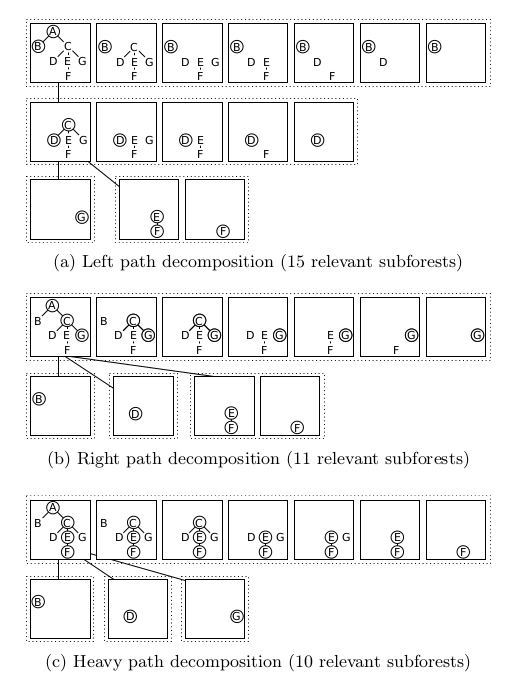
\includegraphics[width=85mm, height=100mm]{../img/LRH_decomposition.png}
\caption{Celková dekompozícia pomocou LRH strategií \citenum{RTED}}
\label{obr:LRH_decomposition}
\end{figure}

Nasledujúca lemma, ktorú pre $heavy$ cesty dokázali \citet{DMRW}
a pre $left$ cesty zase \citet{ZHANGSHASHA}
\footnote{Pre $right$ cesty to platí obdobne, stačí nám zmeniť poradie medzi potomkami vrcholov}
nám ukáže, že počet problémov ktoré potrebujeme vyrátať závisí od výberu dekompozičnej stratégie.

\begin{lemma}
  Počet podproblémov (relevant subproblems) počítaných $SinglePath$ funkciou pre dvojicu
  stromov $F$ a $G$ je rovná
  \begin{align*}
    \# = 
    \begin{cases}
      \abs{F} \times \abs{\FrelevantSubforests(G, \Gamma^{L}(G))} & \text{pre $left$ cesty}
      \\
      \abs{F} \times \abs{\FrelevantSubforests(G, \Gamma^{R}(G))} & \text{pre $right$ cesty}
      \\
      \abs{F} \times \abs{\AfullDecomposition(G)} & \text{pre $heavy$ cesty}
    \end{cases}
  \end{align*}
\end{lemma}

\begin{lemma}
  Minimálny počet podproblémov (cena počítania danou stratégiou),
  ktoré potrebujeme vyrátať pri použití GTEDu je
  \begin{align*}
    cena(F, G) = min
    \begin{cases}
      \abs{F} \times \abs{\AfullDecomposition(G)} &+ \rtedCostSum{F}{H}{G}
      \\
      \abs{G} \times \abs{\AfullDecomposition(F)} &+ \rtedCostSum{G}{H}{F}
      \\
      \abs{F} \times \abs{\FrelevantSubforests(G, \Gamma^{L}(G))} &+ \rtedCostSum{F}{L}{G}
      \\
      \abs{G} \times \abs{\FrelevantSubforests(F, \Gamma^{L}(F))} &+ \rtedCostSum{G}{L}{F}
      \\
      \abs{F} \times \abs{\FrelevantSubforests(G, \Gamma^{R}(G))} &+ \rtedCostSum{F}{R}{G}
      \\
      \abs{G} \times \abs{\FrelevantSubforests(F, \Gamma^{R}(F))} &+ \rtedCostSum{G}{R}{F}
    \end{cases}
  \end{align*}
  pričom $\Gamma^{L}$ a $\Gamma^{R}$ sú funkcie vracajúce $left$ a $right$ cestu v lese.
\end{lemma}

\begin{dukaz}
  Je uvedený v \citenum{RTED}
\end{dukaz}

Popíšeme algoritmus \ref{alg:rted} - RTED, od tvorcov \citet{RTED}.
Vďaka jeho rýchlosti \O{$n^2$} si optimálnu stratégiu nájdeme a aj vypočítame
$GTED$ v čase \O{$n^3$}.

\begin{algorithm}
  \caption{Optimal strategy}
  \label{alg:rted}
  \begin{algorithmic}[1]
    \Procedure {rted}{$F, G$}
      \State $L_{v}, R_{v}, H_{v} \gets$ arrays $\abs{F} \times \abs{G}$
      \State $L_{w}, R_{w}, H_{w} \gets$ arrays $\abs{G}$
      \ForAll {$v$ postorder in $F$}
        \ForAll {$w$ postorder in $G$}
          \If {$v$ is leaf}
            \State $L_{v}[v, w] \gets R_{v}[v, w] \gets H_{v}[v, w] \gets 0$
          \EndIf
          \If {$w$ is leaf}
            \State $L_{w}[w] \gets R_{w}[w] \gets  H_{w}[w] \gets 0$
          \EndIf

          \State $C := \set{$
            \Indent
              \State $(\abs{F_{v}} \times \AfullDecomposition(G_{w}) +
                H_{v}[v, w], \gamma^{H}(F)),$
              \State $(\abs{G_{w}} \times \AfullDecomposition(F_{v}) +
                H_{w}[w], \gamma^{H}(G)),$
              \State $(\abs{F_{v}} \times
                \abs{\FrelevantSubforests(G_{w}, \Gamma^{L}(G))} +
                L_{v}[v, w], \gamma^{L}(F)),$
              \State $(\abs{G_{w}} \times
                \abs{\FrelevantSubforests(F_{v}, \Gamma^{L}(F)}) +
                L_{w}[w], \gamma^{L}(G)),$
              \State $(\abs{F_{v}} \times
                \abs{\FrelevantSubforests(G_{w}, \Gamma^{R}(G))} +
                R_{v}[v, w], \gamma^{R}(F)),$
              \State $(\abs{G_{w}} \times
                \abs{\FrelevantSubforests(F_{v}, \Gamma^{R}(F))} +
                R_{w}[w], \gamma^{R}(G))$
              \State $}$
            \EndIndent

            \State Get $(c_{min}, \gamma_{min}) \in C$ such that
              $c_{min} = min \set{c' | (c', \gamma') \in C}$
            \State $Strategies[v, w] := \gamma_{min}$

            \If {$v$ is not root of tree}
            \State \Call{update}{$L_{v}$, v, w, $c_{min}$, $\gamma^{L}(parent(v)$}
              \State \Call{update}{$R_{v}$, v, w, $c_{min}$, $\gamma^{R}(parent(v)$}
              \State \Call{update}{$H_{v}$, v, w, $c_{min}$, $\gamma^{H}(parent(v)$}
            \EndIf
            \If {$w$ is not root of tree}
              \State \Call{update}{$L_{w}$, w, $c_{min}$, $\gamma^{L}(parent(w)$}
              \State \Call{update}{$R_{w}$, w, $c_{min}$, $\gamma^{R}(parent(w)$}
              \State \Call{update}{$H_{w}$, w, $c_{min}$, $\gamma^{H}(parent(w)$}
            \EndIf
        \EndFor
      \EndFor
      \State \Return {$Strategies$}
    \EndProcedure

  \item[]

    \Procedure {update}{$Table, v, w, c_{min}, \gamma$}
      \State $Table[parent(v), w] \pluseq
        \begin{cases}
          Table[v, w] & \text{if $v \in \gamma$}
          \\
          c_{min} & \text{otherwise}
        \end{cases}$
    \EndProcedure

    \Procedure {update}{$Table, w, c_{min}, \gamma$}
      \State $Table[parent(w)] \quad \pluseq
        \begin{cases}
          Table[w] & \quad \text{if $v \in \gamma$}
          \\
          c_{min} & \quad \text{otherwise}
        \end{cases}$
    \EndProcedure
  \end{algorithmic}
\end{algorithm}

Algoritmus prechádza vrcholmi stromov a spočíta si, aká je optimálna dekompozičná stratégia
pre danú dvojicu podstromov, teda pri akej potrebujem vyrátať minimálny počet podproblémov.

Stromom prechádza v postorder poradí, teda najprv navštívi potomkov zľava doprava, a až tak
samotný vrchol.
Toto poradie je zvolené kvôli tomu, aby sa znížila pamäťová náročnosť a nemuseli ukladať hodnoty
medzi všetkými dvojicami podstromov. Namiesto toho inkrementujeme hodnotu v rodičovskom vrchole
(procedúry $Update$) pri každej návšteve jeho potomka.

\begin{lemma}
  Algoritmus \ref{alg:rted} vyráta optimalnú LRH stratégiu pre dvojicu podstromov $F$ a $G$ a
  časová náročnosť algoritmu je \O{$n^2$}.
\end{lemma}

\begin{dukaz}
  Je uvedený v \citet{RTED}.
\end{dukaz}


\newcommand{\degree}{\ensuremath{^{\circ}}}

\chapter{Kreslenie molekuly}

Po tom čo získame a aplikujeme mapovanie medzi šablonovou a cieľovou molekulou RNA,
ziskame cieľovú molekulu s čiastočnou vizualizáciou, ktorej zvyšok treba dopočitať.

Po operáciach delete ostávajú v molekule prázdne diery, naopak po insertoch potrebujeme
vypočítať, kam umiestnime bázový pár, resp. samotnú bázu, prípadne ešte potrebujeme pre
ňu urobiť miesto. Update vrcholu v strome nerobí žiadne štruktúrne zmeny, zmení sa iba
názov bázy na danom mieste.

Sekundárna štruktúra RNA obsahuje množstvo motivov popisaných na obrázku \ref{obr:RNA_motifs}.
Vo všeobecnosti ale sa každý z týchto motivov skladá zo stemu a loopu.

Stemom budeme ďalej nazývať časť RNA, ktorá zodpovedá vnútornému vrcholu v strome. Loop
budeme označovať listy v RNA strome (lese), nezáleží či je to bulge, interior loop, hairpin
alebo multibranch loop, ako aj ukazuje obrázok \ref{obr:RNA_motifs_stem_loop}.

Stem začína vždy v najvyššom vrchole stromu (v smere ku koreňu), ktorý je zároveň vnútorným
vrcholom a nemá žiadnych súrodencov, ktorý by boli rovnako vnútornými vrcholmi.
To znamená, že do multibranch loop vchádza 1 stem (ten tu konci) a vychádza z nej niekoľko nových stemov.
Naopak pre bulge a interior loop jeden stem vchádza do štruktúry ale pokračuje ďalej.

\begin{figure}[H]
\centering
\fbox{
\includegraphics[trim=0.3cm 24.7cm 17cm 2cm]{../img/stem_loop-colored}}
\caption{Rozlisenie stemov a loopov v molekule: cierne su stemy, farebne odlisene su bazy patriace do jednej loopy}
\label{obr:RNA_motifs_stem_loop}
\end{figure}

\section{Štruktúry v RNA}

V článku od \citet{RNA_DRAW} autori popisujú pravidlá vizualizácie sekundárnej štruktúry RNA.

Nakreslenie musí byť rovinné bez krížení, bázy tvoriace rôzne druhy loopov musia ležať na kružniciach
a bázy tvoriace stem majú ležať na priamke.
Ďalším pravidlom je, že vzdialenosť medzi bázami má byť konštantná, či už vzdialenosť medzi bázami jedného páru,
alebo bázami sekvencie.

Ako je ukázane na obrázku \ref{obr:RNA_full}, pravidla niesu niekedy rešpektované. To zťažuje pouzitie obrazka
ako šablony, kedže vo výslednom obrázku chceme všetky tieto pravidlá rešpektovať.

\section{Algoritmus}
Čiastočnej vizualizácie, ktorú dostávame z mapovania sa chceme dotýkať čo najmenej. To znamená,
že všetky zásahy sa snažíme robiť iba v miestach, ktoré boli dotknuté vkladaním alebo mazaním báz.

Jediné výnimky sú normalizácia vzdialensti medzi bázovými pármi a vyrovnávanie stemov.

\subsection{Normalizácia vzdialeností v bázových pároch a vyrovnavanie stemov}

Ako bolo uvedené, stemom rozumieme nevetviacu sa časť stromu tvorenú iba bázovými pármi.

Algoritmus normalizácie vzdialeností medzi vrcholmi bázových párov stojí iba v preiterovaní celého stromu
a ak nejaké párové vrcholy sú od seba príliž vzdialené, priblíži ich k sebe.

Vyrovnávací algoritmus prechádza všetky stemy. Z ich začiatkov vedie priamku, na ktorej majú byť podľa pravidla uložené
všetky stemove vrcholy. Rotáciami a posunutiami podstromov vieme docieliť to, aby vrcholy stemu na tejto priamke ležali.

% TODO obrázok vyrovnávania

\subsection{Operácie na stromoch}

Čitateľa zoznámime s 2 operáciami, ktoré budeme vykonávať na molekule. Tie budeme používať nezávisle
na tom, či vrcholy do stromu vkladáme alebo mažeme.

\begin{algorithm}
  \caption{Rozloženie báz na kružnicu}
  \label{alg:operácia_circle_reinsert}
  \begin{algorithmic}[1]
    \Procedure {rozlozBazy}{Begin, End, Bases}
      \State $n \gets$ veľkosť zoznamu báz $Bases$
      \State $\Gamma \gets$ dostatočne veľká kružnica pre $n$ bodov prechádzajúca bodmi $Begin$ a $End$
      \State $\Pi \gets$ rozdel kruhový obluk kružnice $\Gamma$ od $Begin$ po $End$ na $n$ bodov
      \ForAll{$i$ in 1 .. $n$}
        \State nastav pozíciu bázy $Bases[i]$ na bod $\Pi[i]$
      \EndFor
    \EndProcedure
  \end{algorithmic}
\end{algorithm}

\begin{algorithm}
  \caption{Posunutie podstromu}
  \label{alg:operacia_tree_shift}
  \begin{algorithmic}[1]
    \Procedure {posunPodstrom}{Root, Vector}
      \ForAll {vrchol $V$ v podstrome vrcholu $Root$}
        \If {vrchol $V$ už má určenu pozíciu, t.j. nieje práve vložený}
          \State pripočítaj k pozicií bázy $V$ vektor $Vector$
        \EndIf
      \EndFor
    \EndProcedure
  \end{algorithmic}
\end{algorithm}

Ako sme písali už skôr, všetky loop štruktúry majú byť uložené na kružniciach. K tomu nám pomôže funkcia
\ref{alg:operacia_circle_reinsert}. Tá dostáva na vstupe zoznam báz $Bases$ a dva body v rovine, $Begin$ a $End$.
Týmito bodmi potrebujeme viesť kružnicu, ktorá bude dostatočne veľká, teda aby na ňu všetky bázy zo zoznamu vošli.
Veľkosťou kružnice v tomto prípade myslíme dĺžku kruhového obluku medzi vrcholmi $Begin$ a $End$.

V našom programe používame iteračný algoritmus, ktorý ju pomaly zväčšuje alebo zmenšuje.
Nakoniec buď nájde kružnicu, ktorej veľkosť je optimálna, alebo ani na maximálny počet krokov takú kružnicu nenájde
a tak vráti tu z posledného kroku. Na obrázku \ref{obr:insert_circle_hairpin} vidíme celý algoritmus zväčšovania kružnice.

\begin{figure}
  \begin{subfigure}{0.3\textwidth}
    \fbox{
\includegraphics[trim=1cm 24.5cm 17cm 2.5cm]{../img/alg-insert/circle-small}}
  \end{subfigure}
  \begin{subfigure}{0.3\textwidth}
    \fbox{
\includegraphics[trim=1cm 24.5cm 17cm 2.5cm]{../img/alg-insert/circle-big}}
  \end{subfigure}
  \begin{subfigure}{0.3\textwidth}
    \fbox{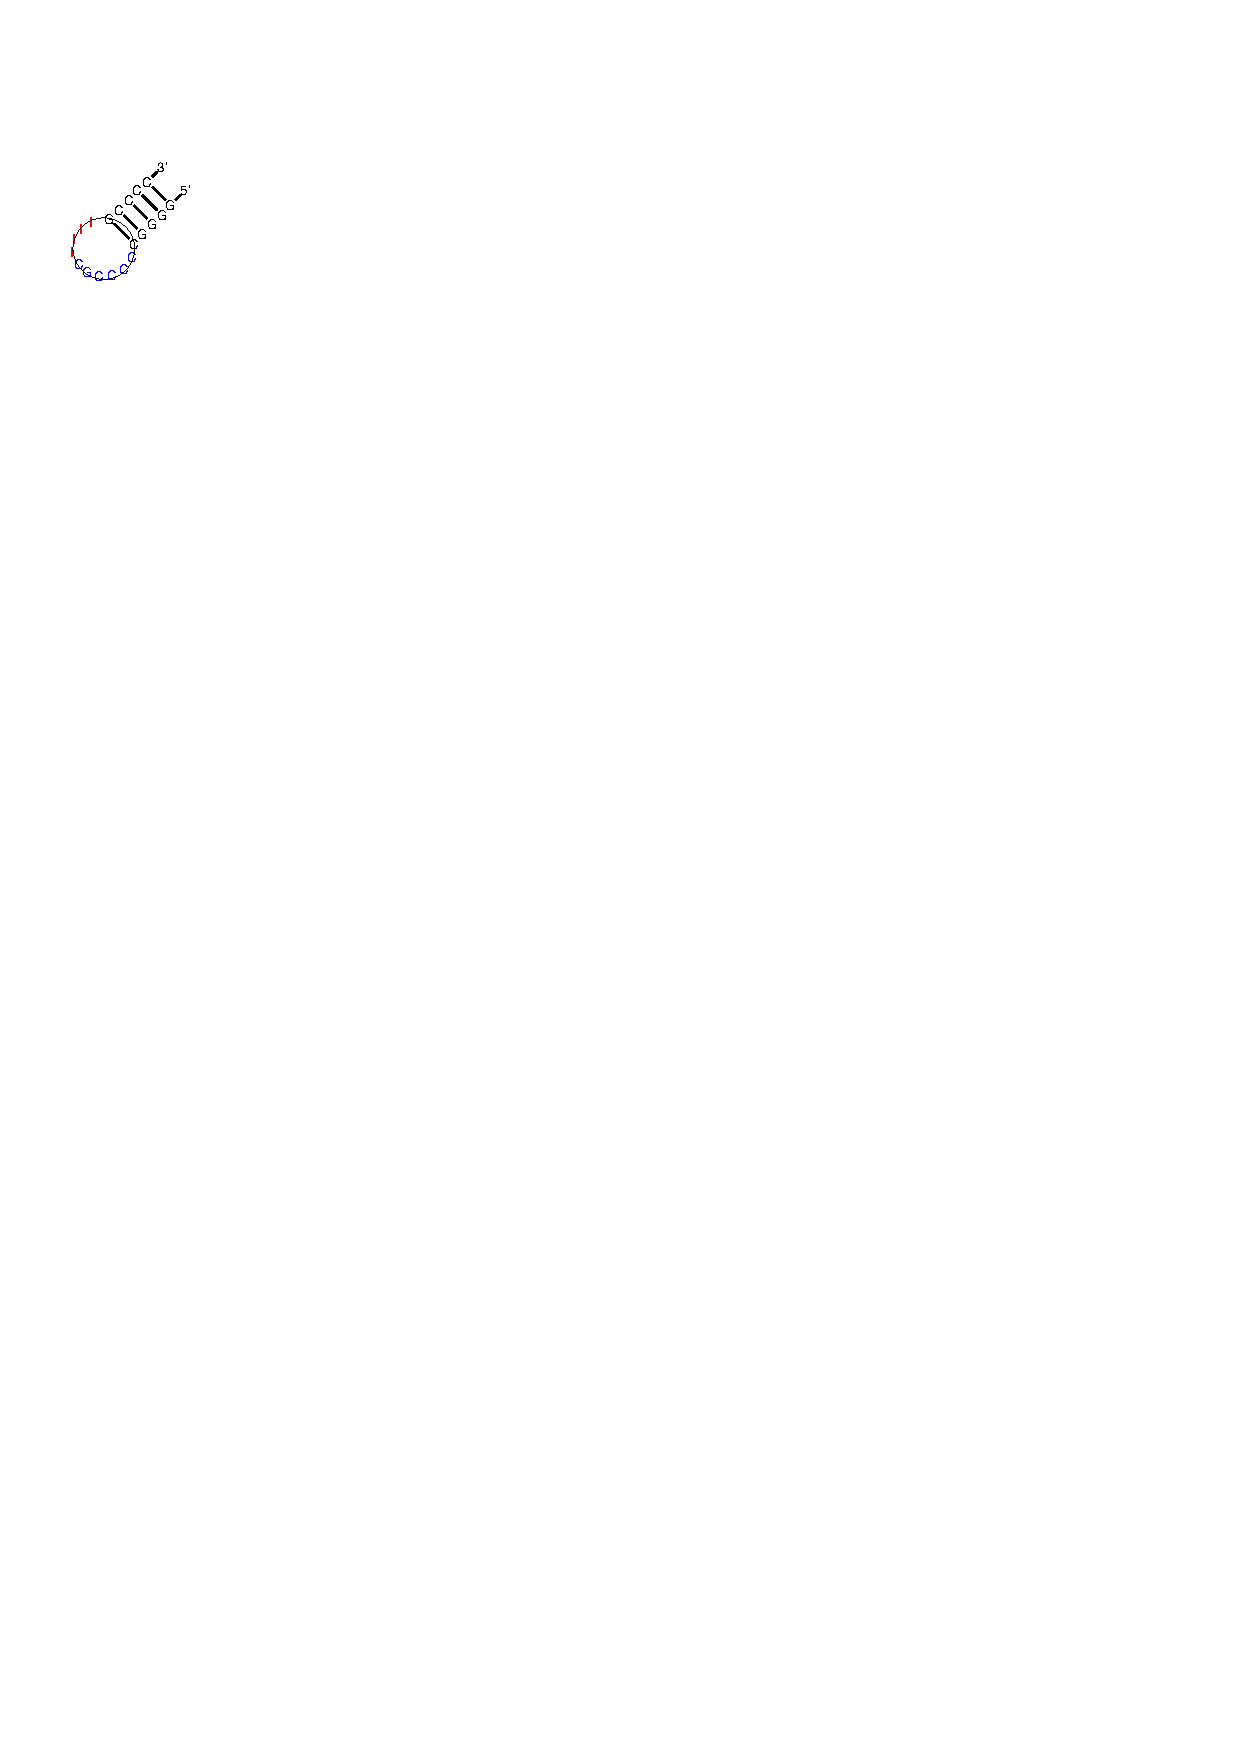
\includegraphics[trim=1cm 24.5cm 17cm 2.5cm]{../img/alg-insert/alg-insert/circle-big-end}}
  \end{subfigure}

  \caption{Priklad zvacsovania kruznice a insertu do hairpinu}
  \label{obr:insert_circle_hairpin}
\end{figure}

Operácia v rámci algoritmu \ref{alg:operacia_tree_shift} nám pomôže urobiť miesto na novo vložené bázové páry,
alebo naopak ak sme niečo zmazali, tak dokáže celý podstrom pritiahnuť späť.

\subsection{Vkladanie nového vrcholu do stromu}

Pri vkladaní nového vrcholu do stromu môžu nastať nasledovné možnosti.

Ak vkladáme list do hairpinu, je to jednodúche, potrebujeme iba použiť procedúru z algoritmu \ref{alg:operacia_circle_reinsert}
s parametrami $Begin = $ požicia prvej bázy z bázového páru, $End = $ požičia druhej bázy z páru
a $Bases = $ zoznam všetkých potomkov.

Trochu zložitejšie je to pri vkladaní listu do stemu. V tomto prípade buď už stem obsahoval nejaký loop, alebo vzniká nová.
Najprv potrebujeme upraviť vzdialenosť medzi vrcholmi stemu, teda posunuť celý podstrom aby nám dané bázy vošli.
To vyriešime algoritmom \ref{alg:operacia_tree_shift}. Následne nájdeme kružnicu a bázy na ňu naukladáme.

Vkladanie bázového páru do stemu je jednoduché. Najprv posunieme celý podstrom a urobíme tak miesto pre novú dvojicu
báz, a potom ich uložíme na pozíciu kde by mala patriť. Môže sa stať, že vložením vrcholu do stemu zdedíme niekoľko
listov z predka. V tomto prípade iba použijeme operáciu vloženia vrcholu a updatu loopov pred aj za vloženým vrcholom.

\subsection{Modifikácia multibrach loop}

Modifikácia multibranch loop je zložitejšia ako všetky predchádzajúce prípady. Obrázky sú väčšinou ručné upravené tak,
aby bol čo najkompaktnejší a kvôli tomu sa často nerešpektujú pravidlá o kružnicovom tvare štruktúry.
Kvôli tomu sa snažíme do tejto štruktúry nezasahovať, ak sa to dá.

Prekresleniu celej štruktúry sa môžeme vyhnúť napríklad pri zmene počtu listov medzi jednotlivými vetvami.
Ak je zmena dostatočne malá, môžeme vrcholy roztiahnuť, alebo naopak priblížiť k sebe.

Ak sa jedná o pridanie/odobratie celej vetvy stromu, modifikácií sa nevyhneme. V tom prípade potrebujeme
rozdistribuovať všetky vrcholy patriace do loop na kružnicu. Je to podobný proces ako sa používa iba pre samotné loopy,
ale potrebujeme posúvať celé podstromy a zrotovať ich správnym smerom.

\subsection{Mazanie vrcholu zo stromu}

Mazanie považujeme za inverznú operáciu voči vkladaniu do stromu. Vzhľadom k tomu, používame rovnaké operácie
rozdistribuovania vrcholov v loope, alebo posúvanie podstromu, ktoré sa deje v tomto prípade opačným smerom
k predkovi.


%%% Fiktivní kapitola s ukázkami sazby

\chapter{Nápověda k~sazbě}

\section{Úprava práce}

Vlastní text bakalářské práce je uspořádaný hierarchicky do kapitol a podkapitol,
každá kapitola začíná na nové straně. Text je zarovnán do bloku. Nový odstavec
se obvykle odděluje malou vertikální mezerou a odsazením prvního řádku. Grafická
úprava má být v~celém textu jednotná.

Práce se tiskne na bílý papír formátu A4. Okraje musí ponechat dost místa na vazbu:
doporučen je horní, dolní a pravý okraj $25\,\rm mm$, levý okraj $40\,\rm mm$.
Číslují se všechny strany kromě obálky a informačních stran na začátku práce;
první číslovaná strana bývá obvykle ta s~obsahem.

Písmo se doporučuje dvanáctibodové ($12\,\rm pt$) se standardní vzdáleností mezi řádky
(pokud píšete ve Wordu nebo podobném programu, odpovídá tomu řádkování $1,5$; v~\TeX{}u
není potřeba nic přepínat). Pro běžný text používejte vzpřímené patkové písmo.
Text matematických vět se obvykle tiskne pro zdůraznění skloněným (slanted) písmem,
není-li k~dispozici, může být zastoupeno kurzívou.

Primárně je doporučován jednostranný tisk (příliš tenkou práci lze obtížně svázat).
Delší práce je lepší tisknout oboustranně a přizpůsobit tomu velikosti okrajů:
$40\,\rm mm$ má vždy \emph{vnitřní} okraj. Rub titulního listu zůstává nepotištěný.

Zkratky použité v textu musí být vysvětleny vždy u prvního výskytu zkratky (v~závorce nebo
v poznámce pod čarou, jde-li o složitější vysvětlení pojmu či zkratky). Pokud je zkratek
více, připojuje se seznam použitých zkratek, včetně jejich vysvětlení a/nebo odkazů
na definici.

Delší převzatý text jiného autora je nutné vymezit uvozovkami nebo jinak vyznačit a řádně
citovat.

\section{Jednoduché příklady}

Čísla v~českém textu obvykle sázíme v~matematickém režimu s~desetinnou čárkou:
%%% Bez \usepackage{icomma}:
% $\pi \doteq 3{,}141\,592\,653\,589$.
%%% S \usepackage{icomma}:
$\pi \doteq 3,141\,592\,653\,589$.
V~matematických textech se považuje za přípustné používat desetinnou tečku
(pro lepší odlišení od čárky v~roli oddělovače). Numerické výsledky se uvádějí
s~přiměřeným počtem desetinných míst.

Mezi číslo a jednotku patří úzká mezera: šířka stránky A4 činí $210\,\rm mm$, což si
pamatuje pouze $5\,\%$ autorů. Pokud ale údaj slouží jako přívlastek, mezeru vynecháváme:
$25\rm mm$ okraj, $95\%$ interval spolehlivosti.

Rozlišujeme různé druhy pomlček:
červeno-černý (krátká pomlčka),
strana 16--22 (střední),
$45-44$ (matematické minus),
a~toto je --- jak se asi dalo čekat --- vložená věta ohraničená dlouhými pomlčkami.

V~českém textu se používají \uv{české} uvozovky, nikoliv ``anglické''.

% V tomto odstavci se vlnka zviditelňuje
{
\def~{{\tt\char126}}
Na některých místech je potřeba zabránit lámání řádku (v~\TeX{}u značíme vlnovkou):
u~předložek (neslabičnych, nebo obecně jednopísmenných), vrchol~$v$, před $k$~kroky,
a~proto, \dots{} obecně kdekoliv, kde by při rozlomení čtenář \uv{škobrtnul}.
}

\section{Matematické vzorce a výrazy}

Proměnné sázíme kurzívou (to \TeX{} v~matematickém módu dělá sám, ale
nezapomínejte na to v~okolním textu a také si matematický mód zapněte).
Názvy funkcí sázíme vzpřímeně. Tedy například:
$\var(X) = \E X^2 - \bigl(\E X \bigr)^2$.

Zlomky uvnitř odstavce (třeba $\frac{5}{7}$ nebo $\frac{x+y}{2}$) mohou
být příliš stísněné, takže je lepší sázet jednoduché zlomky s~lomítkem:
$5/7$, $(x+y)/2$.

Nechť
\[   % LaTeXová náhrada klasického TeXového $$
\mathbb{X} = \begin{pmatrix}
      \T{\bm x_1} \\
      \vdots \\
      \T{\bm x_n}
      \end{pmatrix}.
\]
Povšimněme si tečky za~maticí. Byť je matematický text vysázen
ve~specifickém prostředí, stále je gramaticky součástí věty a~tudíž je
zapotřebí neopomenout patřičná interpunkční znaménka. Výrazy, na které
chceme později odkazovat, je vhodné očíslovat:
\begin{equation}\label{eq01:Xmat}
\mathbb{X} = \begin{pmatrix}
      \T{\bm x_1} \\
      \vdots \\
      \T{\bm x_n}
      \end{pmatrix}.
\end{equation}
Výraz \eqref{eq01:Xmat} definuje matici $\mathbb{X}$. Pro lepší čitelnost
a~přehlednost textu je vhodné číslovat pouze ty výrazy, na které se
autor někde v~další části textu odkazuje. To jest, nečíslujte
automaticky všechny výrazy vysázené některým z~matematických
prostředí.

Zarovnání vzorců do několika sloupečků:
\begin{alignat*}{3}
S(t) &= \pr(T > t),    &\qquad t&>0       &\qquad&\text{ (zprava spojitá),}\\
F(t) &= \pr(T \leq t), &\qquad t&>0       &\qquad&\text{ (zprava spojitá).}
\end{alignat*}

Dva vzorce se spojovníkem:
\begin{equation}\label{eq01:FS}
\left.
\begin{aligned}
S(t) &= \pr(T > t) \\[1ex]
F(t) &= \pr(T \leq t)
\end{aligned}
\;	% zde pomůže ručně vynechat trochu místa
\right\}
\quad t>0 \qquad \text{(zprava spojité).}
\end{equation}

Dva centrované nečíslované vzorce:
\begin{gather*}
\bm Y = \mathbb{X}\bm\beta + \bm\varepsilon, \\[1ex]
\mathbb{X} = \begin{pmatrix} 1 & \T{\bm x_1} \\ \vdots & \vdots \\ 1 &
  \T{\bm x_n} \end{pmatrix}.
\end{gather*}
Dva centrované číslované vzorce:
\begin{gather}
\bm Y = \mathbb{X}\bm\beta + \bm\varepsilon, \label{eq02:Y}\\[1ex]
\mathbb{X} = \begin{pmatrix} 1 & \T{\bm x_1} \label{eq03:X}\\ \vdots & \vdots \\ 1 &
  \T{\bm x_n} \end{pmatrix}.
\end{gather}

Definice rozdělená na dva případy:
\[
P_{r-j}=
\begin{cases}
0, & \text{je-li $r-j$ liché},\\
r!\,(-1)^{(r-j)/2}, & \text{je-li $r-j$ sudé}.
\end{cases}
\]
Všimněte si použití interpunkce v této konstrukci. Čárky a tečky se
dávají na místa, kam podle jazykových pravidel patří.

\begin{align}
x& = y_1-y_2+y_3-y_5+y_8-\dots = && \text{z \eqref{eq02:Y}} \nonumber\\
& = y'\circ y^* = && \text{podle \eqref{eq03:X}} \nonumber\\
& = y(0) y' && \text {z Axiomu 1.}
\end{align}


Dva zarovnané vzorce nečíslované:
\begin{align*}
L(\bm\theta) &= \prod_{i=1}^n f_i(y_i;\,\bm\theta), \\
\ell(\bm\theta) &= \log\bigl\{L(\bm\theta)\bigr\} =
\sum_{i=1}^n \log\bigl\{f_i(y_i;\,\bm\theta)\bigr\}.
\end{align*}
Dva zarovnané vzorce, první číslovaný:
\begin{align}
L(\bm\theta) &= \prod_{i=1}^n f_i(y_i;\,\bm\theta), \label{eq01:L} \\
\ell(\bm\theta) &= \log\bigl\{L(\bm\theta)\bigr\} =
\sum_{i=1}^n \log\bigl\{f_i(y_i;\,\bm\theta)\bigr\}. \nonumber
\end{align}

Vzorec na dva řádky, první řádek zarovnaný vlevo, druhý vpravo, nečíslovaný:
\begin{multline*}
\ell(\mu,\,\sigma^2) = \log\bigl\{L(\mu,\,\sigma^2)\bigr\} =
\sum_{i=1}^n \log\bigl\{f_i(y_i;\,\mu,\,\sigma^2)\bigr\}= \\
  = -\,\frac{n}{2}\,\log(2\pi\sigma^2) \,-\,
\frac{1}{2\sigma^2}\sum_{i=1}^n\,(y_i - \mu)^2.
\end{multline*}

Vzorec na dva řádky, zarovnaný na $=$, číslovaný uprostřed:
\begin{equation}\label{eq01:ell}
\begin{split}
\ell(\mu,\,\sigma^2) &= \log\bigl\{L(\mu,\,\sigma^2)\bigr\} =
\sum_{i=1}^n \log\bigl\{f(y_i;\,\mu,\,\sigma^2)\bigr\}= \\
& = -\,\frac{n}{2}\,\log(2\pi\sigma^2) \,-\,
\frac{1}{2\sigma^2}\sum_{i=1}^n\,(y_i - \mu)^2.
\end{split}
\end{equation}

\section{Definice, věty, důkazy, \dots}

Konstrukce typu definice, věta, důkaz, příklad, \dots je vhodné
odlišit od okolního textu a~případně též číslovat s~možností použití
křížových odkazů. Pro každý typ těchto konstrukcí je vhodné mít
v~souboru s~makry (\texttt{makra.tex}) nadefinované jedno prostředí,
které zajistí jak vizuální odlišení od okolního textu, tak
automatické číslování s~možností křížově odkazovat.

\begin{definice}\label{def01:1}
  Nechť náhodné veličiny $X_1,\dots,X_n$ jsou definovány na témž
  prav\-dě\-po\-dob\-nost\-ním prostoru $(\Omega,\,\mathcal{A},\,\pr)$. Pak
  vektor $\bm X = \T{(X_1,\dots,X_n)}$ nazveme \emph{náhodným
    vektorem}.
\end{definice}

\begin{definice}[náhodný vektor]\label{def01:2}
  Nechť náhodné veličiny $X_1,\dots,X_n$ jsou definovány na témž
  pravděpodobnostním prostoru $(\Omega,\,\mathcal{A},\,\pr)$. Pak
  vektor $\bm X = \T{(X_1,\dots,X_n)}$ nazveme \emph{náhodným
    vektorem}.
\end{definice}
Definice~\ref{def01:1} ukazuje použití prostředí pro sazbu definice
bez titulku, definice~\ref{def01:2} ukazuje použití prostředí pro
sazbu definice s~titulkem.

\begin{veta}\label{veta01:1}
  Náhodný vektor $\bm X$ je měřitelné zobrazení prostoru
  $(\Omega,\,\mathcal{A},\,\pr)$ do $(\R_n,\,\mathcal{B}_n)$.
\end{veta}

\begin{lemma}[\citealp{Andel07}, str. 29]\label{veta01:2}
  Náhodný vektor $\bm X$ je měřitelné zobrazení prostoru
  $(\Omega,\,\mathcal{A},\,\pr)$ do $(\R_n,\,\mathcal{B}_n)$.
\end{lemma}
\begin{dukaz}
  Jednotlivé kroky důkazu jsou podrobně popsány v~práci \citet[str.
  29]{Andel07}.
\end{dukaz}
Věta~\ref{veta01:1} ukazuje použití prostředí pro sazbu matematické
věty bez titulku, lemma~\ref{veta01:2} ukazuje použití prostředí pro
sazbu matematické věty s~titulkem. Lemmata byla zavedena v~hlavním
souboru tak, že sdílejí číslování s~větami.






%%% Fiktivní kapitola s ukázkami citací

\chapter{Odkazy na literaturu}

Odkazy na literaturu vytváříme nejlépe pomocí příkazů
\verb|\citet|, \verb|\citep| atp.
(viz {\LaTeX}ový balíček \textsf{natbib}) a~následného použití
Bib{\TeX}u. V~matematickém textu obvykle odkazujeme stylem \uv{Jméno
autora/autorů (rok vydání)}, resp. \uv{Jméno autora/autorů [číslo
odkazu]}. V~českém/slovenském textu je potřeba se navíc vypořádat
s~nutností skloňovat jméno autora, respektive přechylovat jméno
autorky. Je potřeba mít na paměti, že standardní příkazy
\verb|\citet|, \verb|\citep|
produkují referenci se jménem autora/autorů v~prvním pádě a~jména
autorek jsou nepřechýlena.

Pokud nepoužíváme bib\TeX{}, řídíme se normou ISO 690 a zvyklostmi
oboru.

Jména časopisů lze uvádět zkráceně, ale pouze v~kodifikované podobě.

\section{Několik ukázek}

Mezi nejvíce citované statistické články patří práce Kaplana a~Meiera a~Coxe
\citep{KaplanMeier58, Cox72}. \citet{Student08} napsal článek o~t-testu.

Prof. Anděl je autorem učebnice matematické statistiky
\citep[viz][]{Andel98}. Teorii odhadu se věnuje práce
\citet{LehmannCasella98}. V~případě odkazů na specifickou informaci
(definice, důkaz, \dots) uvedenou v~knize bývá užitečné uvést
specificky číslo kapitoly, číslo věty atp. obsahující požadovanou
informaci, např. viz \citet[Věta 4.22]{Andel07} nebo \citep[viz][Věta
4.22]{Andel07}.

Mnoho článků je výsledkem spolupráce celé řady osob. Při odkazování
v~textu na článek se třemi autory obvykle při prvním výskytu uvedeme
plný seznam: \citet*{DempsterLairdRubin77} představili koncept EM
algoritmu. Respektive: Koncept EM algoritmu byl představen v~práci
Dempstera, Lairdové a~Rubina \citep*{DempsterLairdRubin77}. Při každém
dalším výskytu již používáme zkrácenou verzi:
\citet{DempsterLairdRubin77} nabízejí též několik příkladů použití EM
algoritmu. Respektive: Několik příkladů použití EM algoritmu lze
nalézt též v~práci Dempstera a~kol. \citep{DempsterLairdRubin77}.

U~článku s~více než třemi autory odkazujeme vždy zkrácenou formou:
První výsledky projektu ACCEPT jsou uvedeny v~práci Genbergové a~kol.
\citep{Genberget08}. V~textu \emph{nenapíšeme}: První výsledky
projektu ACCEPT jsou uvedeny v~práci \citet*{Genberget08}.






%%% Fiktivní kapitola s ukázkami tabulek, obrázků a kódu

\chapter{Tabulky, obrázky, programy}

Používání tabulek a grafů v~odborném textu má některá společná
pravidla a~některá specifická. Tabulky a grafy neuvádíme přímo do
textu, ale umístíme je buď na samostatné stránky nebo na vyhrazené
místo v~horní nebo dolní části běžných stránek. \LaTeX\ se o~umístění
plovoucích grafů a tabulek postará automaticky.

Každý graf a tabulku
očíslujeme a umístíme pod ně legendu. Legenda má popisovat obsah grafu
či tabulky tak podrobně, aby jim čtenář rozuměl bez důkladného
studování textu práce.

Na každou tabulku a graf musí být v~textu odkaz
pomocí jejich čísla. Na příslušném místě textu pak shrneme ty
nejdůležitější závěry, které lze z~tabulky či grafu učinit. Text by
měl být čitelný a srozumitelný i~bez prohlížení tabulek a grafů a
tabulky a grafy by měly být srozumitelné i~bez podrobné četby textu.

Na tabulky a grafy odkazujeme pokud možno nepřímo v~průběhu běžného
toku textu; místo \emph{\uv{Tabulka~\ref{tab03:Nejaka} ukazuje, že
    muži jsou v~průměru o~$9,9\,\rm kg$ těžší než ženy}} raději napíšeme
\emph{\uv{Muži jsou o~$9,9\,\rm kg$ těžší než ženy (viz
    Tabulka~\ref{tab03:Nejaka})}}.

\section{Tabulky}

\begin{table}[b!]

\centering
%%% Tabulka používá následující balíčky:
%%%   - booktabs (\toprule, \midrule, \bottomrule)
%%%   - dcolumn (typ sloupce D: vycentrovaná čísla zarovnaná na
%%%     desetinnou čárku
%%%     Všimněte si, že ve zdrojovém kódu jsou desetinné tečky, ale
%%%     tisknou se čárky.
%%% Dále používáme příkazy \pulrad a \mc definované v makra.tex

\begin{tabular}{l@{\hspace{1.5cm}}D{.}{,}{3.2}D{.}{,}{1.2}D{.}{,}{2.3}}
\toprule
 & \mc{} & \mc{\textbf{Směrod.}} & \mc{} \\
\pulrad{\textbf{Efekt}} & \mc{\pulrad{\textbf{Odhad}}} & \mc{\textbf{chyba}$^a$} &
\mc{\pulrad{\textbf{P-hodnota}}} \\
\midrule
Abs. člen     & -10.01 & 1.01 & \mc{---} \\
Pohlaví (muž) & 9.89   & 5.98 & 0.098 \\
Výška (cm)    & 0.78   & 0.12 & <0.001 \\
\bottomrule
\multicolumn{4}{l}{\footnotesize \textit{Pozn:}
$^a$ Směrodatná chyba odhadu metodou Monte Carlo.}
\end{tabular}

\caption{Maximálně věrohodné odhady v~modelu M.}\label{tab03:Nejaka}

\end{table}

U~\textbf{tabulek} se doporučuje dodržovat následující pravidla:

\begin{itemize} %% nebo compactitem z balíku paralist
\item Vyhýbat se svislým linkám. Silnějšími vodorovnými linkami
  oddělit tabulku od okolního textu včetně legendy, slabšími
  vodorovnými linkami oddělovat záhlaví sloupců od těla tabulky a
  jednotlivé části tabulky mezi sebou. V~\LaTeX u tuto podobu tabulek
  implementuje balík \texttt{booktabs}. Chceme-li výrazněji oddělit
  některé sloupce od jiných, vložíme mezi ně větší mezeru.
\item Neměnit typ, formát a význam obsahu políček v~tomtéž sloupci
  (není dobré do téhož sloupce zapisovat tu průměr, onde procenta).
\item Neopakovat tentýž obsah políček mnohokrát za sebou. Máme-li
  sloupec \textit{Rozptyl}, který v~prvních deseti řádcích obsahuje
  hodnotu $0,5$ a v~druhých deseti řádcích hodnotu $1,5$, pak tento
  sloupec raději zrušíme a vyřešíme to jinak. Například můžeme tabulku
  rozdělit na dvě nebo do ní vložit popisné řádky, které informují
o~nějaké proměnné hodnotě opakující se v~následujícím oddíle tabulky
  (např. \emph{\uv{Rozptyl${}=0,5$}} a níže \emph{\uv{Rozptyl${}=
      1,5$}}).
\item Čísla v~tabulce zarovnávat na desetinnou čárku.
\item V~tabulce je někdy potřebné používat zkratky, které se jinde
nevyskytují. Tyto zkratky můžeme vysvětlit v~legendě nebo
v~poznámkách pod tabulkou. Poznámky pod tabulkou můžeme využít i
k~podrobnějšímu vysvětlení významu  některých sloupců nebo hodnot.
\end{itemize}

\section{Obrázky}

Několik rad týkajících se obrázků a grafů.

\begin{itemize}
\item Graf by měl být vytvořen ve velikosti, v~níž bude použit
  v~práci. Zmenšení příliš velkého grafu vede ke špatné čitelnosti
  popisků.
\item Osy grafu musí být řádně popsány ve stejném jazyce, v~jakém je
  psána práce (absenci diakritiky lze tolerovat). Kreslíme-li graf
  hmotnosti proti výšce, nenecháme na nich popisky \texttt{ht} a
  \texttt{wt}, ale osy popíšeme \emph{Výška [cm]} a~\emph{Hmotnost
    [kg]}. Kreslíme-li graf funkce $h(x)$, popíšeme osy $x$ a $h(x)$.
  Každá osa musí mít jasně určenou škálu.
\item Chceme-li na dvourozměrném grafu vyznačit velké množství bodů,
  dáme pozor, aby se neslily do jednolité černé tmy. Je-li bodů mnoho,
  zmenšíme velikost symbolu, kterým je vykreslujeme, anebo vybereme
  jen malou část bodů, kterou do grafu zaneseme. Grafy, které obsahují
  tisíce bodů, dělají problémy hlavně v~elektronických dokumentech,
  protože výrazně zvětšují velikost souborů.
\item Budeme-li práci tisknout černobíle, vyhneme se používání barev.
  Čáry roz\-li\-šu\-je\-me typem (plná, tečkovaná, čerchovaná,\ldots), plochy
  dostatečně roz\-díl\-ný\-mi intensitami šedé nebo šrafováním. Význam
  jednotlivých typů čar a~ploch vysvětlíme buď v~textové legendě ke
  grafu anebo v~grafické legendě, která je přímo součástí obrázku.
\item Vyhýbejte se bitmapovým obrázkům o~nízkém rozlišení a zejména
  JPEGům (zuby a kompresní artefakty nevypadají na papíře pěkně).
  Lepší je vytvářet obrázky vektorově a vložit do textu jako PDF.
\end{itemize}

\section{Programy}

Algoritmy, výpisy programů a popis interakce s~programy je vhodné
odlišit od ostatního textu. Jednou z~možností je použití {\LaTeX}o\-vé\-ho balíčku
\texttt{fancyvrb} (fancy verbatim), pomocí něhož je v~souboru \texttt{makra.tex}
nadefinováno prostředí \texttt{code}. Pomocí něho lze vytvořit
např. následující ukázky.

\begin{code}
> mean(x)
[1] 158.90
> objekt$prumer
[1] 158.90
\end{code}
%$
Menší písmo:
\begin{code}[fontsize=\footnotesize]
> mean(x)
[1] 158.90
> objekt$prumer
[1] 158.90
\end{code}
%$
Bez rámečku:
\begin{code}[frame=none]
> mean(x)
[1] 158.90
> objekt$prumer
[1] 158.90
\end{code}
%$
Užší rámeček:
\begin{code}[xrightmargin=20em]
> mean(x)
[1] 158.90
> objekt$prumer
[1] 158.90
\end{code}
%$


\chapter*{Záver}
\addcontentsline{toc}{chapter}{Záver}

V rámci práce sme vytvorili program TRAVeLer umožňujúci
vizualizáciu sekundárnej štruktúry RNA pomocou existujúceho
obrázka molekuly, ktorý nám slúži ako predloha.

Stromová reprezentácia štruktúry a~následné
použitie \textit{tree-edit-distance} metriky podobnosti dvoch
štruktúr sa ukázali ako správna voľba.
Algoritmus TED nám nie len dá informáciu o tom,
s ako vzdialenými štruktúrami pracujeme, ale dáva nám
aj návod, ako transformovať šablónovú molekulu na tu cieľovú.
U dostatočne podobných štruktúr nám už namapovaná štruktúra
ukáže aké častí sú spoločné a ktoré sa líšia a dá nám
predstavu, ako bude výsledná vizualizácia vyzerať.

Výsledky ukazujú, že ak použijeme štruktúrne dostatočne blízku
molekulu ako šablónu, výsledok vizualizácie je uspokojujúci.
S väčšou vzdialenosťou ale počet prekryvov vo výsledných obrázkoch
stúpa.

V budúcnosti bude vhodné upraviť naše primitívne kresliace algoritmy.
Takýmto vylepšením by bola implementácia otáčania vetiev RNA stromov,
v prípade, že sme našli prekryv.
Druhou možnosťou by bolo pridanie interaktívneho nástroja na úpravu
vzniknutých obrázkov. Ten by umožnil ručne upraviť výsledné vizualizácie.

V našej práci sme sa úplne vyhli pseudouzlom. To nám umožnilo
reprezentovať sekundárnu štruktúru RNA ako usporiadaný, zakorenený strom.
Avšak, pseudouzly sú jej dôležitou súčasťou.
Možným vylepšením by preto bolo, zohľadniť ich existenciu pri mapovaní.
To si ale bude vyžadovať hlbšiu analýzu tohoto problému.

Program bol uvolnený pre používanie biológmi. Budeme očakávať ich reakcie,
na základe ktorých budeme implementovať ďalšie vylepšenia programu.
Dúfame, že aplikácia nájde cestu k svojím používateľom.



%%% Seznam použité literatury
%%% Seznam použité literatury (bibliografie)
%%%
%%% Pro vytváření bibliografie používáme bibTeX. Ten zpracovává
%%% citace v textu (např. makro \cite{...}) a vyhledává k nim literaturu
%%% v souboru literatura.bib.
%%%
%%% Příkaz \bibliographystyle určuje, jakým stylem budou citovány odkazy
%%% v textu. V závorce je název zvoleného souboru .bst. Styly plainnat
%%% a unsrt jsou standardní součástí latexových distribucí. Styl czplainnat
%%% je dodáván s touto šablonou a bibTeX ho hledá v aktuálním adresáři.

\bibliographystyle{czplainnat}    %% Autor (rok) s českými spojkami
% \bibliographystyle{plainnat}    %% Autor (rok) s anglickými spojkami
% \bibliographystyle{unsrt}       %% [číslo]

\renewcommand{\bibname}{Seznam použité literatury}

%%% Vytvoření seznamu literatury. Pozor, pokud jste necitovali ani jednu
%%% položku, seznam se automaticky vynechá.

\bibliography{literatura}

%%% Kdybyste chtěli bibliografii vytvářet ručně (bez bibTeXu), lze to udělat
%%% následovně. V takovém případě se řiďte normou ISO 690 a zvyklostmi v oboru.

% \begin{thebibliography}{99}
%
% \bibitem{lamport94}
%   {\sc Lamport,} Leslie.
%   \emph{\LaTeX: A Document Preparation System}.
%   2. vydání.
%   Massachusetts: Addison Wesley, 1994.
%   ISBN 0-201-52983-1.
%
% \end{thebibliography}


%%% Obrázky v bakalářské práci
%%% (pokud jich je malé množství, obvykle není třeba seznam uvádět)
\listoffigures

%%% Tabulky v bakalářské práci (opět nemusí být nutné uvádět)
%%% U matematických prací může být lepší přemístit seznam tabulek na začátek práce.
\listoftables

%%% Použité zkratky v bakalářské práci (opět nemusí být nutné uvádět)
%%% U matematických prací může být lepší přemístit seznam zkratek na začátek práce.
\chapwithtoc{Seznam použitých zkratek}

%%% Přílohy k bakalářské práci, existují-li. Každá příloha musí být alespoň jednou
%%% odkazována z vlastního textu práce. Přílohy se číslují.
%%%
%%% Do tištěné verze se spíše hodí přílohy, které lze číst a prohlížet (dodatečné
%%% tabulky a grafy, různé textové doplňky, ukázky výstupů z počítačových programů,
%%% apod.). Do elektronické verze se hodí přílohy, které budou spíše používány
%%% v elektronické podobě než čteny (zdrojové kódy programů, datové soubory,
%%% interaktivní grafy apod.). Elektronické přílohy se nahrávají do SISu a lze
%%% je také do práce vložit na CD/DVD.
\chapwithtoc{Přílohy}

\openright
\end{document}
